% Options for packages loaded elsewhere
\PassOptionsToPackage{unicode}{hyperref}
\PassOptionsToPackage{hyphens}{url}
\PassOptionsToPackage{dvipsnames,svgnames,x11names}{xcolor}
%
\documentclass[
  letterpaper,
  DIV=11,
  numbers=noendperiod]{scrartcl}

\usepackage{amsmath,amssymb}
\usepackage{iftex}
\ifPDFTeX
  \usepackage[T1]{fontenc}
  \usepackage[utf8]{inputenc}
  \usepackage{textcomp} % provide euro and other symbols
\else % if luatex or xetex
  \usepackage{unicode-math}
  \defaultfontfeatures{Scale=MatchLowercase}
  \defaultfontfeatures[\rmfamily]{Ligatures=TeX,Scale=1}
\fi
\usepackage{lmodern}
\ifPDFTeX\else  
    % xetex/luatex font selection
\fi
% Use upquote if available, for straight quotes in verbatim environments
\IfFileExists{upquote.sty}{\usepackage{upquote}}{}
\IfFileExists{microtype.sty}{% use microtype if available
  \usepackage[]{microtype}
  \UseMicrotypeSet[protrusion]{basicmath} % disable protrusion for tt fonts
}{}
\makeatletter
\@ifundefined{KOMAClassName}{% if non-KOMA class
  \IfFileExists{parskip.sty}{%
    \usepackage{parskip}
  }{% else
    \setlength{\parindent}{0pt}
    \setlength{\parskip}{6pt plus 2pt minus 1pt}}
}{% if KOMA class
  \KOMAoptions{parskip=half}}
\makeatother
\usepackage{xcolor}
\setlength{\emergencystretch}{3em} % prevent overfull lines
\setcounter{secnumdepth}{5}
% Make \paragraph and \subparagraph free-standing
\makeatletter
\ifx\paragraph\undefined\else
  \let\oldparagraph\paragraph
  \renewcommand{\paragraph}{
    \@ifstar
      \xxxParagraphStar
      \xxxParagraphNoStar
  }
  \newcommand{\xxxParagraphStar}[1]{\oldparagraph*{#1}\mbox{}}
  \newcommand{\xxxParagraphNoStar}[1]{\oldparagraph{#1}\mbox{}}
\fi
\ifx\subparagraph\undefined\else
  \let\oldsubparagraph\subparagraph
  \renewcommand{\subparagraph}{
    \@ifstar
      \xxxSubParagraphStar
      \xxxSubParagraphNoStar
  }
  \newcommand{\xxxSubParagraphStar}[1]{\oldsubparagraph*{#1}\mbox{}}
  \newcommand{\xxxSubParagraphNoStar}[1]{\oldsubparagraph{#1}\mbox{}}
\fi
\makeatother

\usepackage{color}
\usepackage{fancyvrb}
\newcommand{\VerbBar}{|}
\newcommand{\VERB}{\Verb[commandchars=\\\{\}]}
\DefineVerbatimEnvironment{Highlighting}{Verbatim}{commandchars=\\\{\}}
% Add ',fontsize=\small' for more characters per line
\newenvironment{Shaded}{}{}
\newcommand{\AlertTok}[1]{\textcolor[rgb]{0.75,0.01,0.01}{\textbf{\colorbox[rgb]{0.97,0.90,0.90}{#1}}}}
\newcommand{\AnnotationTok}[1]{\textcolor[rgb]{0.79,0.38,0.79}{#1}}
\newcommand{\AttributeTok}[1]{\textcolor[rgb]{0.00,0.34,0.68}{#1}}
\newcommand{\BaseNTok}[1]{\textcolor[rgb]{0.69,0.50,0.00}{#1}}
\newcommand{\BuiltInTok}[1]{\textcolor[rgb]{0.39,0.29,0.61}{\textbf{#1}}}
\newcommand{\CharTok}[1]{\textcolor[rgb]{0.57,0.30,0.62}{#1}}
\newcommand{\CommentTok}[1]{\textcolor[rgb]{0.54,0.53,0.53}{#1}}
\newcommand{\CommentVarTok}[1]{\textcolor[rgb]{0.00,0.58,1.00}{#1}}
\newcommand{\ConstantTok}[1]{\textcolor[rgb]{0.67,0.33,0.00}{#1}}
\newcommand{\ControlFlowTok}[1]{\textcolor[rgb]{0.12,0.11,0.11}{\textbf{#1}}}
\newcommand{\DataTypeTok}[1]{\textcolor[rgb]{0.00,0.34,0.68}{#1}}
\newcommand{\DecValTok}[1]{\textcolor[rgb]{0.69,0.50,0.00}{#1}}
\newcommand{\DocumentationTok}[1]{\textcolor[rgb]{0.38,0.47,0.50}{#1}}
\newcommand{\ErrorTok}[1]{\textcolor[rgb]{0.75,0.01,0.01}{\underline{#1}}}
\newcommand{\ExtensionTok}[1]{\textcolor[rgb]{0.00,0.58,1.00}{\textbf{#1}}}
\newcommand{\FloatTok}[1]{\textcolor[rgb]{0.69,0.50,0.00}{#1}}
\newcommand{\FunctionTok}[1]{\textcolor[rgb]{0.39,0.29,0.61}{#1}}
\newcommand{\ImportTok}[1]{\textcolor[rgb]{1.00,0.33,0.00}{#1}}
\newcommand{\InformationTok}[1]{\textcolor[rgb]{0.69,0.50,0.00}{#1}}
\newcommand{\KeywordTok}[1]{\textcolor[rgb]{0.12,0.11,0.11}{\textbf{#1}}}
\newcommand{\NormalTok}[1]{\textcolor[rgb]{0.12,0.11,0.11}{#1}}
\newcommand{\OperatorTok}[1]{\textcolor[rgb]{0.79,0.38,0.79}{#1}}
\newcommand{\OtherTok}[1]{\textcolor[rgb]{0.00,0.43,0.16}{#1}}
\newcommand{\PreprocessorTok}[1]{\textcolor[rgb]{0.00,0.43,0.16}{#1}}
\newcommand{\RegionMarkerTok}[1]{\textcolor[rgb]{0.00,0.34,0.68}{\colorbox[rgb]{0.88,0.91,0.97}{#1}}}
\newcommand{\SpecialCharTok}[1]{\textcolor[rgb]{0.24,0.68,0.91}{#1}}
\newcommand{\SpecialStringTok}[1]{\textcolor[rgb]{1.00,0.33,0.00}{#1}}
\newcommand{\StringTok}[1]{\textcolor[rgb]{0.75,0.01,0.01}{#1}}
\newcommand{\VariableTok}[1]{\textcolor[rgb]{0.00,0.34,0.68}{#1}}
\newcommand{\VerbatimStringTok}[1]{\textcolor[rgb]{0.75,0.01,0.01}{#1}}
\newcommand{\WarningTok}[1]{\textcolor[rgb]{0.75,0.01,0.01}{#1}}

\providecommand{\tightlist}{%
  \setlength{\itemsep}{0pt}\setlength{\parskip}{0pt}}\usepackage{longtable,booktabs,array}
\usepackage{calc} % for calculating minipage widths
% Correct order of tables after \paragraph or \subparagraph
\usepackage{etoolbox}
\makeatletter
\patchcmd\longtable{\par}{\if@noskipsec\mbox{}\fi\par}{}{}
\makeatother
% Allow footnotes in longtable head/foot
\IfFileExists{footnotehyper.sty}{\usepackage{footnotehyper}}{\usepackage{footnote}}
\makesavenoteenv{longtable}
\usepackage{graphicx}
\makeatletter
\def\maxwidth{\ifdim\Gin@nat@width>\linewidth\linewidth\else\Gin@nat@width\fi}
\def\maxheight{\ifdim\Gin@nat@height>\textheight\textheight\else\Gin@nat@height\fi}
\makeatother
% Scale images if necessary, so that they will not overflow the page
% margins by default, and it is still possible to overwrite the defaults
% using explicit options in \includegraphics[width, height, ...]{}
\setkeys{Gin}{width=\maxwidth,height=\maxheight,keepaspectratio}
% Set default figure placement to htbp
\makeatletter
\def\fps@figure{htbp}
\makeatother

\KOMAoption{captions}{tableheading}
\makeatletter
\@ifpackageloaded{tcolorbox}{}{\usepackage[skins,breakable]{tcolorbox}}
\@ifpackageloaded{fontawesome5}{}{\usepackage{fontawesome5}}
\definecolor{quarto-callout-color}{HTML}{909090}
\definecolor{quarto-callout-note-color}{HTML}{0758E5}
\definecolor{quarto-callout-important-color}{HTML}{CC1914}
\definecolor{quarto-callout-warning-color}{HTML}{EB9113}
\definecolor{quarto-callout-tip-color}{HTML}{00A047}
\definecolor{quarto-callout-caution-color}{HTML}{FC5300}
\definecolor{quarto-callout-color-frame}{HTML}{acacac}
\definecolor{quarto-callout-note-color-frame}{HTML}{4582ec}
\definecolor{quarto-callout-important-color-frame}{HTML}{d9534f}
\definecolor{quarto-callout-warning-color-frame}{HTML}{f0ad4e}
\definecolor{quarto-callout-tip-color-frame}{HTML}{02b875}
\definecolor{quarto-callout-caution-color-frame}{HTML}{fd7e14}
\makeatother
\makeatletter
\@ifpackageloaded{caption}{}{\usepackage{caption}}
\AtBeginDocument{%
\ifdefined\contentsname
  \renewcommand*\contentsname{Table of contents}
\else
  \newcommand\contentsname{Table of contents}
\fi
\ifdefined\listfigurename
  \renewcommand*\listfigurename{List of Figures}
\else
  \newcommand\listfigurename{List of Figures}
\fi
\ifdefined\listtablename
  \renewcommand*\listtablename{List of Tables}
\else
  \newcommand\listtablename{List of Tables}
\fi
\ifdefined\figurename
  \renewcommand*\figurename{Figure}
\else
  \newcommand\figurename{Figure}
\fi
\ifdefined\tablename
  \renewcommand*\tablename{Table}
\else
  \newcommand\tablename{Table}
\fi
}
\@ifpackageloaded{float}{}{\usepackage{float}}
\floatstyle{ruled}
\@ifundefined{c@chapter}{\newfloat{codelisting}{h}{lop}}{\newfloat{codelisting}{h}{lop}[chapter]}
\floatname{codelisting}{Listing}
\newcommand*\listoflistings{\listof{codelisting}{List of Listings}}
\makeatother
\makeatletter
\makeatother
\makeatletter
\@ifpackageloaded{caption}{}{\usepackage{caption}}
\@ifpackageloaded{subcaption}{}{\usepackage{subcaption}}
\makeatother

\ifLuaTeX
  \usepackage{selnolig}  % disable illegal ligatures
\fi
\usepackage{bookmark}

\IfFileExists{xurl.sty}{\usepackage{xurl}}{} % add URL line breaks if available
\urlstyle{same} % disable monospaced font for URLs
\hypersetup{
  pdftitle={GTAPSSP: SSPs for GTAP Framework},
  pdfauthor={Thiago Simonato},
  colorlinks=true,
  linkcolor={blue},
  filecolor={Maroon},
  citecolor={Blue},
  urlcolor={Blue},
  pdfcreator={LaTeX via pandoc}}


\title{GTAPSSP: SSPs for GTAP Framework}
\author{Thiago Simonato}
\date{2025-01-24}

\begin{document}
\maketitle

\renewcommand*\contentsname{Table of contents}
{
\hypersetup{linkcolor=}
\setcounter{tocdepth}{6}
\tableofcontents
}

\section{Introduction}\label{introduction}

This tutorial demonstrates the utilization of the \emph{gtapssp} package
in R for data processing. It covers various steps such as reading,
transforming, and analyzing data, making it suitable for both beginners
and advanced users.

The package provides optimized and user-friendly functions to download
SSP data, interpolate data using spline and beers methods. The
\emph{gtapssp} functions is accompanied by detailed
\href{https://github.com/tsimonato/gtapssp/raw/master/docs/gtapssp_0.0.0.9000.pdf}{manual},
you can also access this manual by pressing \texttt{F1} on the function
name in \href{https://posit.co/download/rstudio-desktop/}{RStudio}.

\section{Installation}\label{installation}

To use the \emph{gtapssp} package, it's necessary to have \emph{R}
installed on your computer, which can be downloaded from
\href{https://www.r-project.org/}{here}. Additionally, we recommend
downloading \emph{RStudio}, available at
\href{https://posit.co/download/rstudio-desktop/}{here}, which provides
a user-friendly interface to work with \emph{R}.

\begin{tcolorbox}[enhanced jigsaw, leftrule=.75mm, toprule=.15mm, breakable, titlerule=0mm, opacitybacktitle=0.6, colframe=quarto-callout-tip-color-frame, arc=.35mm, bottomtitle=1mm, toptitle=1mm, title=\textcolor{quarto-callout-tip-color}{\faLightbulb}\hspace{0.5em}{R install details}, rightrule=.15mm, colback=white, bottomrule=.15mm, opacityback=0, left=2mm, colbacktitle=quarto-callout-tip-color!10!white, coltitle=black]

R is a versatile programming language, with a focus on statistical
computing. It is a big part of academic research in the social sciences.
R is free and open-source and runs on Windows, Mac OS X, and Linux.

\begin{enumerate}
\def\labelenumi{\arabic{enumi}.}
\tightlist
\item
  Download the R installer from the
  \href{https://cran.r-project.org/}{Comprehensive R Archive Network
  (CRAN)}.
\end{enumerate}

\begin{itemize}
\tightlist
\item
  Choose the appropriate installer for your operating system and
  computer architecture (32-bit or 64-bit).
\item
  If on Mac, you will need to know if you are using an Intel or Apple
  Silicon (M1) processor.
\end{itemize}

\begin{enumerate}
\def\labelenumi{\arabic{enumi}.}
\setcounter{enumi}{1}
\item
  Run the installer and follow the instructions.
\item
  We recommend install \textbf{R Tools}. Many of the packages we will be
  using in this course require R Tools to be installed.

  If you are on Windows:
\end{enumerate}

\begin{itemize}
\item
  Download the latest version of the software from the
  \href{https://cran.r-project.org/bin/windows/Rtools/}{R Tools for
  Windows} page.
\item
  Run the installer and follow the instructions.

  If you are on Mac:
\item
  First, install the Xcode Command Line Tools. Go to the
  \href{https://mac.r-project.org/tools/}{R Tools for Mac} page and
  follow the instructions. Note: the precise instructions will vary
  according to the version of macOS you are using.
\item
  Install the gfortran compiler, as also indicated on the
  \href{https://mac.r-project.org/tools/}{R Tools for Mac} page.
\end{itemize}

\end{tcolorbox}

\begin{tcolorbox}[enhanced jigsaw, leftrule=.75mm, toprule=.15mm, breakable, titlerule=0mm, opacitybacktitle=0.6, colframe=quarto-callout-tip-color-frame, arc=.35mm, bottomtitle=1mm, toptitle=1mm, title=\textcolor{quarto-callout-tip-color}{\faLightbulb}\hspace{0.5em}{Python install details}, rightrule=.15mm, colback=white, bottomrule=.15mm, opacityback=0, left=2mm, colbacktitle=quarto-callout-tip-color!10!white, coltitle=black]

\begin{tcolorbox}[enhanced jigsaw, leftrule=.75mm, toprule=.15mm, breakable, titlerule=0mm, opacitybacktitle=0.6, colframe=quarto-callout-important-color-frame, arc=.35mm, bottomtitle=1mm, toptitle=1mm, title=\textcolor{quarto-callout-important-color}{\faExclamation}\hspace{0.5em}{Important}, rightrule=.15mm, colback=white, bottomrule=.15mm, opacityback=0, left=2mm, colbacktitle=quarto-callout-important-color!10!white, coltitle=black]

Python installation is \textbf{only required} if you plan to download
other versions of SSPs datasets from the IIASA. The \texttt{gtapssp}
package includes a built-in default dataset, so installing Python is
optional unless you wish to access the latest or alternative datasets
from IIASA's API (developed in Python).

\end{tcolorbox}

Python is a general-purpose programming language that is becoming
increasingly popular in the social sciences. It is free and open-source
and runs on Windows, Mac OS X, and Linux.

\begin{enumerate}
\def\labelenumi{\arabic{enumi}.}
\item
  Download Python from the
  \href{https://www.python.org/downloads/}{Python Software Foundation}.
\item
  Run the installer and make sure to check the box that says ``Add
  Python to PATH'' before clicking on ``Install Now''.\\
  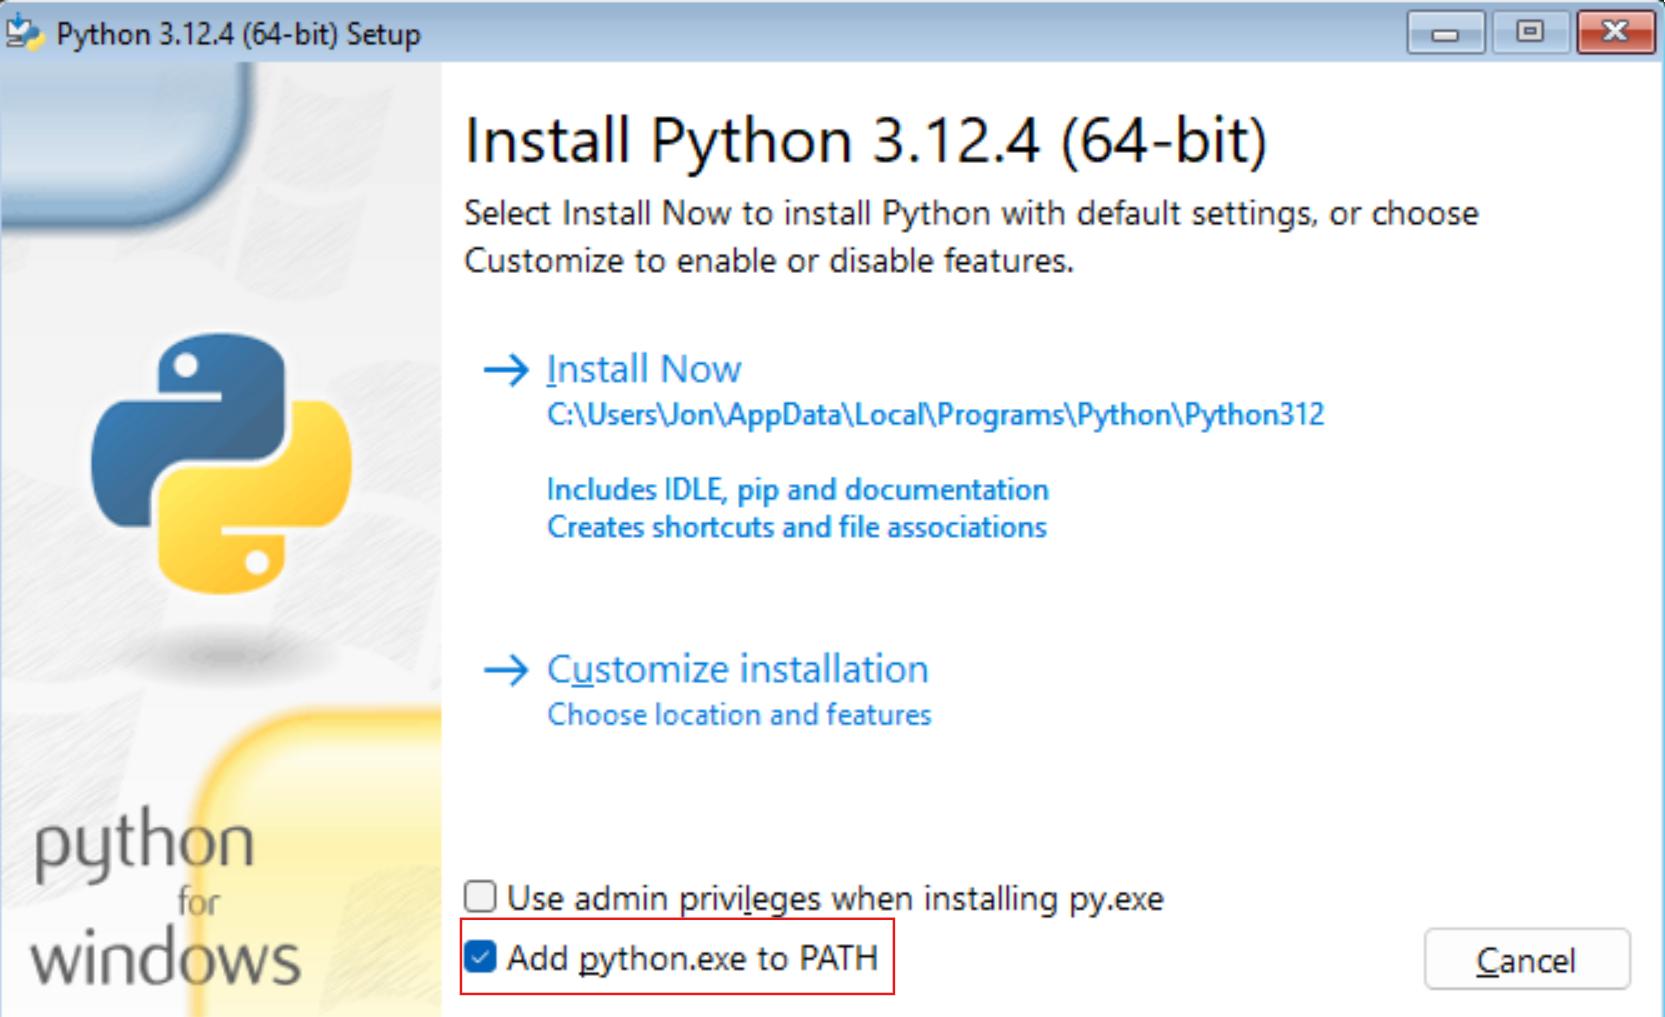
\includegraphics[width=4.94792in,height=\textheight]{images/clipboard-1705657641.png}
\end{enumerate}

\end{tcolorbox}

\begin{tcolorbox}[enhanced jigsaw, leftrule=.75mm, toprule=.15mm, breakable, titlerule=0mm, opacitybacktitle=0.6, colframe=quarto-callout-tip-color-frame, arc=.35mm, bottomtitle=1mm, toptitle=1mm, title=\textcolor{quarto-callout-tip-color}{\faLightbulb}\hspace{0.5em}{IDE install details}, rightrule=.15mm, colback=white, bottomrule=.15mm, opacityback=0, left=2mm, colbacktitle=quarto-callout-tip-color!10!white, coltitle=black]

We recommend RStudio as IDE for R.

\href{https://posit.co/download/rstudio-desktop/}{RStudio} is by far the
most popular IDE used by R programmers. It is free and open-source and
comes with a console and syntax-highlighting editor that supports direct
code execution, as well as tools for plotting, history, debugging, and
workspace management.

\textbf{Alternative}: If you are already familiar with
\href{https://code.visualstudio.com/}{Visual Studio Code (VS Code)}, say
because you have already used it for Python, you can also use it for R
programming. You will need to do a bit of configuration to get it to
work, though. If you choose to use VS Code, download and install the
\href{https://marketplace.visualstudio.com/items?itemName=Ikuyadeu.r}{R
Extension for Visual Studio Code} and remember to follow the
instructions on the \emph{Getting Started} section of the extension
page.

\end{tcolorbox}

You can install the development version of \emph{gtapssp} from
\href{https://github.com/tsimonato/gtapssp}{GitHub} with:

\begin{Shaded}
\begin{Highlighting}[]
\CommentTok{\# If the devtools package is not already installed, please run the disabled line below.}
\CommentTok{\# install.packages("devtools")}

\NormalTok{devtools}\SpecialCharTok{::}\FunctionTok{install\_github}\NormalTok{(}\StringTok{"tsimonato/gtapssp"}\NormalTok{)}
\end{Highlighting}
\end{Shaded}

\section{One-Line Workflow}\label{one-line-workflow}

If you'd like to execute the entire pipeline described in this tutorial
with minimal effort, you can use the \texttt{gtapssp::iiasa\_gtap()}
function. This function runs all steps, including data aggregation,
interpolation, expansion, label merging, and optional file exports.

Here's an example:

\begin{Shaded}
\begin{Highlighting}[]
\NormalTok{ssp\_data }\OtherTok{\textless{}{-}}\NormalTok{ gtapssp}\SpecialCharTok{::}\FunctionTok{iiasa\_gtap}\NormalTok{()}

\NormalTok{ssp\_data}
\end{Highlighting}
\end{Shaded}

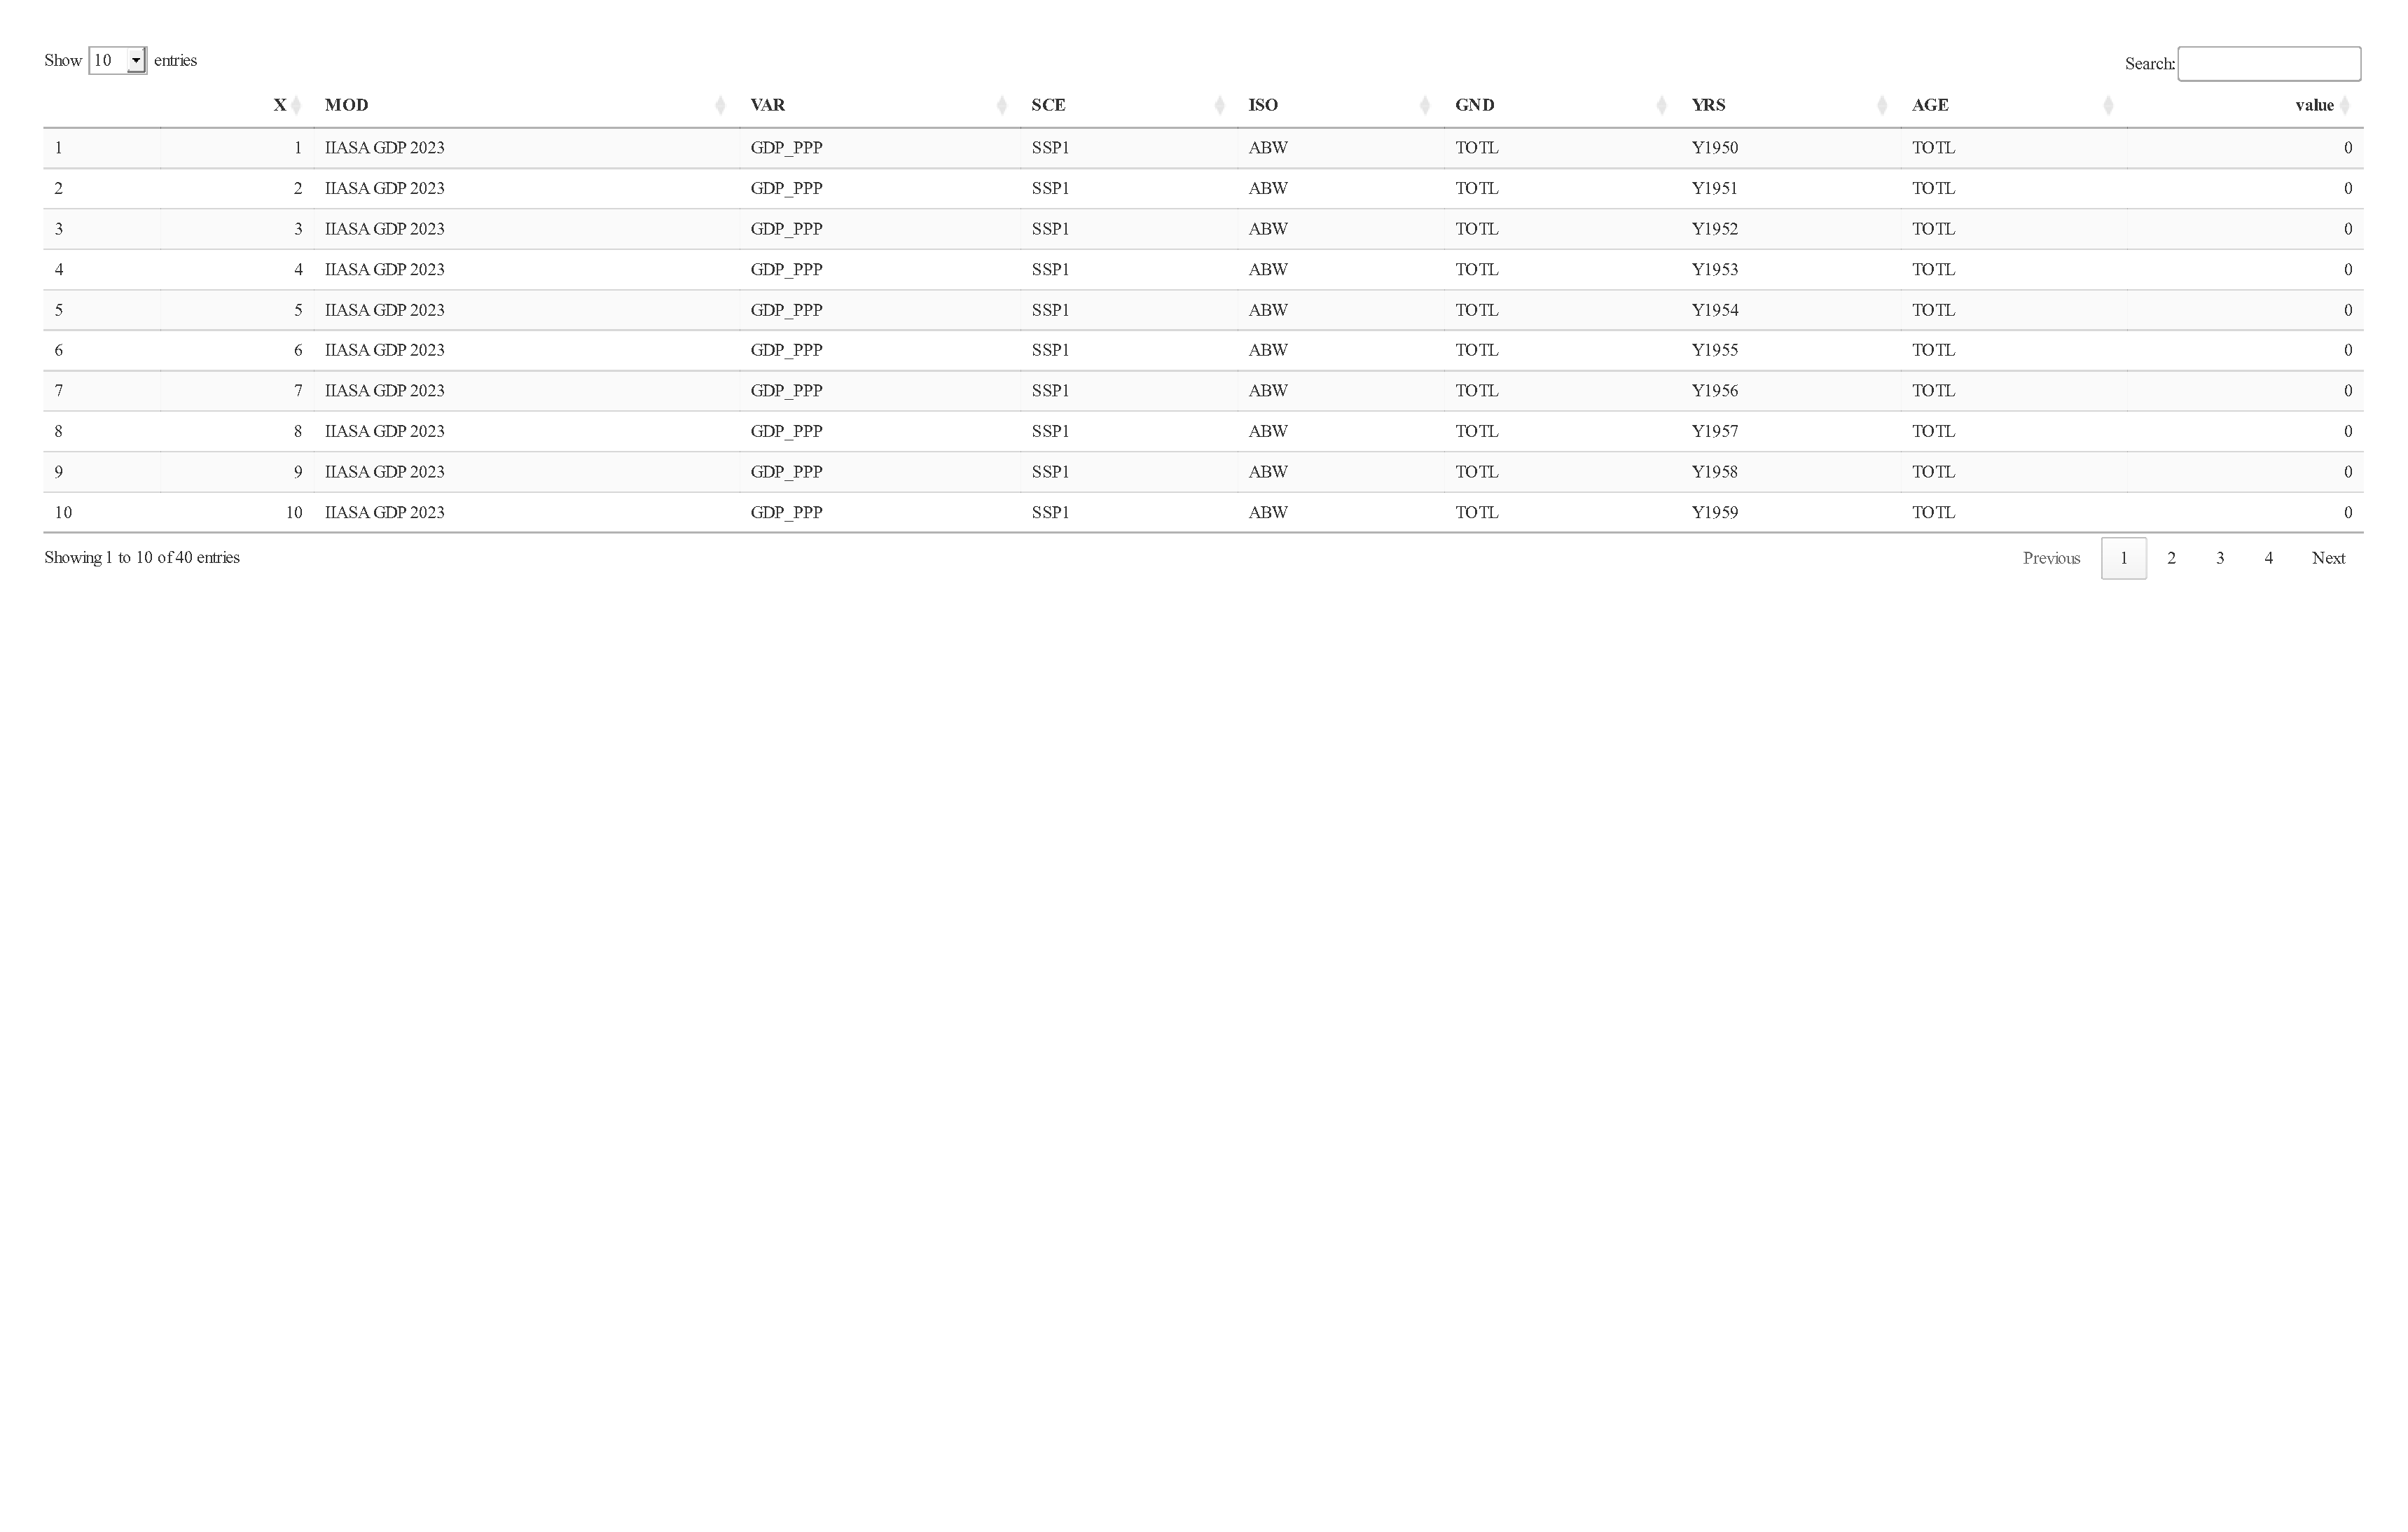
\includegraphics{index_files/figure-pdf/unnamed-chunk-4-1.pdf}

This function provides flexibility to either return the processed
dataset for further use in R or save the output in .har or .csv formats:

\begin{Shaded}
\begin{Highlighting}[]
\CommentTok{\# Run the entire pipeline and save the output as a .HAR file}
\NormalTok{gtapssp}\SpecialCharTok{::}\FunctionTok{iiasa\_gtap}\NormalTok{(}\AttributeTok{outFile =} \StringTok{"gtap\_ssp.har"}\NormalTok{)}
\CommentTok{\# Or save as a .CSV file}
\NormalTok{gtapssp}\SpecialCharTok{::}\FunctionTok{iiasa\_gtap}\NormalTok{(}\AttributeTok{outFile =} \StringTok{"gtap\_ssp.csv"}\NormalTok{)}
\end{Highlighting}
\end{Shaded}

\subsection{Population}

Below is a spatial representation of the population data. The map below
highlights population estimates for females, aged 65 and above in the
year 1950, under the SSP1 scenario. The data is sourced from the
IIASA-WiC POP 2023 dataset.

\begin{Shaded}
\begin{Highlighting}[]
\CommentTok{\# If the gtaptools package is not already installed, please run the disabled line below.}
\CommentTok{\# devtools::install\_github("tsimonato/gtaptools")}
\NormalTok{data\_map  }\OtherTok{\textless{}{-}}\NormalTok{ ssp\_data }\SpecialCharTok{|\textgreater{}} 
\NormalTok{  dplyr}\SpecialCharTok{::}\FunctionTok{mutate}\NormalTok{(}\AttributeTok{iso\_a3 =}\NormalTok{ ISO) }\SpecialCharTok{|\textgreater{}} 
\NormalTok{  dplyr}\SpecialCharTok{::}\FunctionTok{filter}\NormalTok{(MOD }\SpecialCharTok{==} \StringTok{"IIASA{-}WiC POP 2023"}\NormalTok{,}
\NormalTok{                SCE }\SpecialCharTok{==} \StringTok{"SSP1"}\NormalTok{,}
\NormalTok{                GND }\SpecialCharTok{==} \StringTok{"FEML"}\NormalTok{,}
\NormalTok{                AGE }\SpecialCharTok{==} \StringTok{"P65UP"}\NormalTok{,}
\NormalTok{                YRS }\SpecialCharTok{==} \StringTok{"Y1950"}\NormalTok{)}
\CommentTok{\# Example: Plot a map using the \textasciigrave{}plot\_map\textasciigrave{} function}
\NormalTok{gtaptools}\SpecialCharTok{::}\FunctionTok{plot\_map}\NormalTok{(}
  \AttributeTok{input\_data =}\NormalTok{ data\_map,       }\CommentTok{\# Your data frame}
  \AttributeTok{value\_var =} \StringTok{"value"}\NormalTok{,    }\CommentTok{\# Replace with the column name for numeric values to plot}
  \AttributeTok{colors =} \StringTok{"viridis"}\NormalTok{,}
  \AttributeTok{legend\_title =} \StringTok{"Million people"}\NormalTok{,        }\CommentTok{\# Replace with a title for your legend}
\NormalTok{)}
\end{Highlighting}
\end{Shaded}

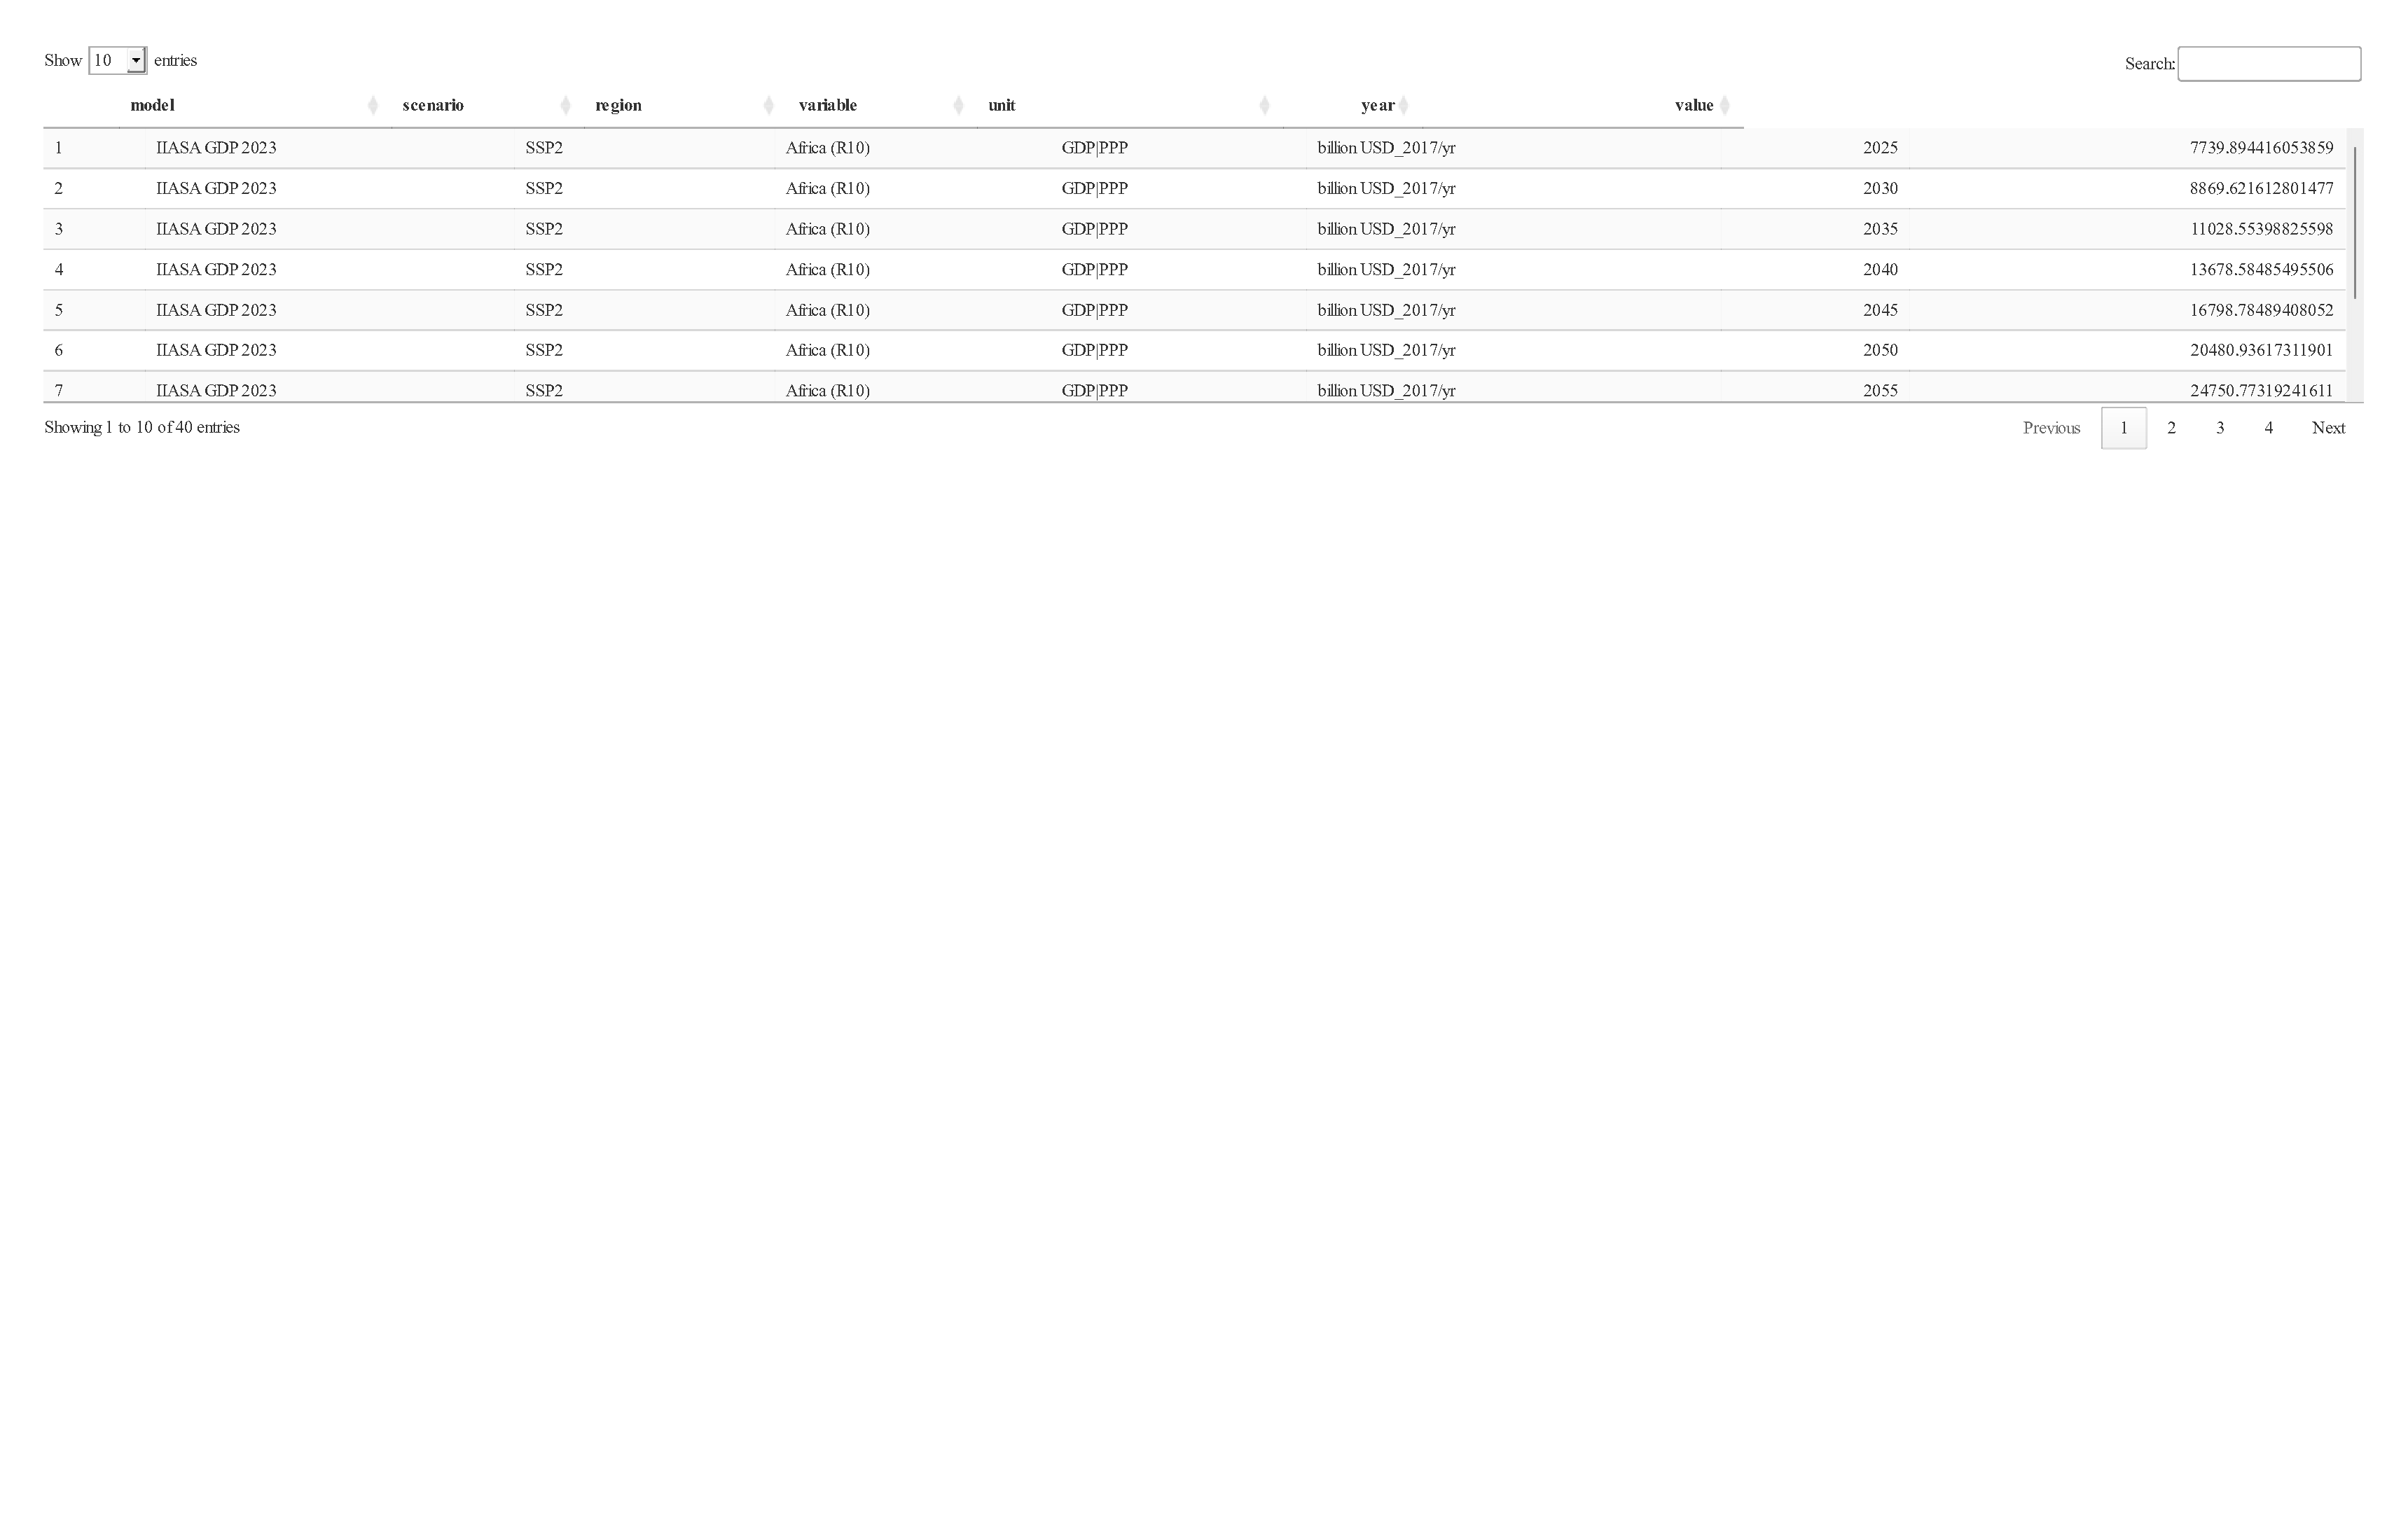
\includegraphics{index_files/figure-pdf/unnamed-chunk-6-1.pdf}

\subsection{GDP per capita}

Below is a spatial representation of GDP per capita projections. The map
below shows GDP per capita in PPP (2017 USD) for the year 2100 under the
SSP1 scenario. The data comes from the OECD ENV-Growth 2023 dataset.

\begin{Shaded}
\begin{Highlighting}[]
\CommentTok{\# If the gtaptools package is not already installed, please run the disabled line below.}
\CommentTok{\# devtools::install\_github("tsimonato/gtaptools")}
\NormalTok{data\_map  }\OtherTok{\textless{}{-}}\NormalTok{ ssp\_data }\SpecialCharTok{|\textgreater{}} 
\NormalTok{  dplyr}\SpecialCharTok{::}\FunctionTok{mutate}\NormalTok{(}\AttributeTok{iso\_a3 =}\NormalTok{ ISO) }\SpecialCharTok{|\textgreater{}} 
\NormalTok{  dplyr}\SpecialCharTok{::}\FunctionTok{filter}\NormalTok{(MOD }\SpecialCharTok{==} \StringTok{"OECD ENV{-}Growth 2023"}\NormalTok{,}
\NormalTok{                VAR }\SpecialCharTok{==} \StringTok{"GDP\_PER\_CAPI"}\NormalTok{,}
\NormalTok{                SCE }\SpecialCharTok{==} \StringTok{"SSP1"}\NormalTok{,}
\NormalTok{                YRS }\SpecialCharTok{==} \StringTok{"Y2100"}\NormalTok{)}
\CommentTok{\# Example: Plot a map using the \textasciigrave{}plot\_map\textasciigrave{} function}
\NormalTok{gtaptools}\SpecialCharTok{::}\FunctionTok{plot\_map}\NormalTok{(}
  \AttributeTok{input\_data =}\NormalTok{ data\_map,       }\CommentTok{\# Your data frame}
  \AttributeTok{value\_var =} \StringTok{"value"}\NormalTok{,    }\CommentTok{\# Replace with the column name for numeric values to plot}
  \AttributeTok{colors =} \StringTok{"viridis"}\NormalTok{,}
  \AttributeTok{legend\_title =} \StringTok{"(PPP, USD 2017)"}\NormalTok{,        }\CommentTok{\# Replace with a title for your legend}
\NormalTok{)}
\end{Highlighting}
\end{Shaded}

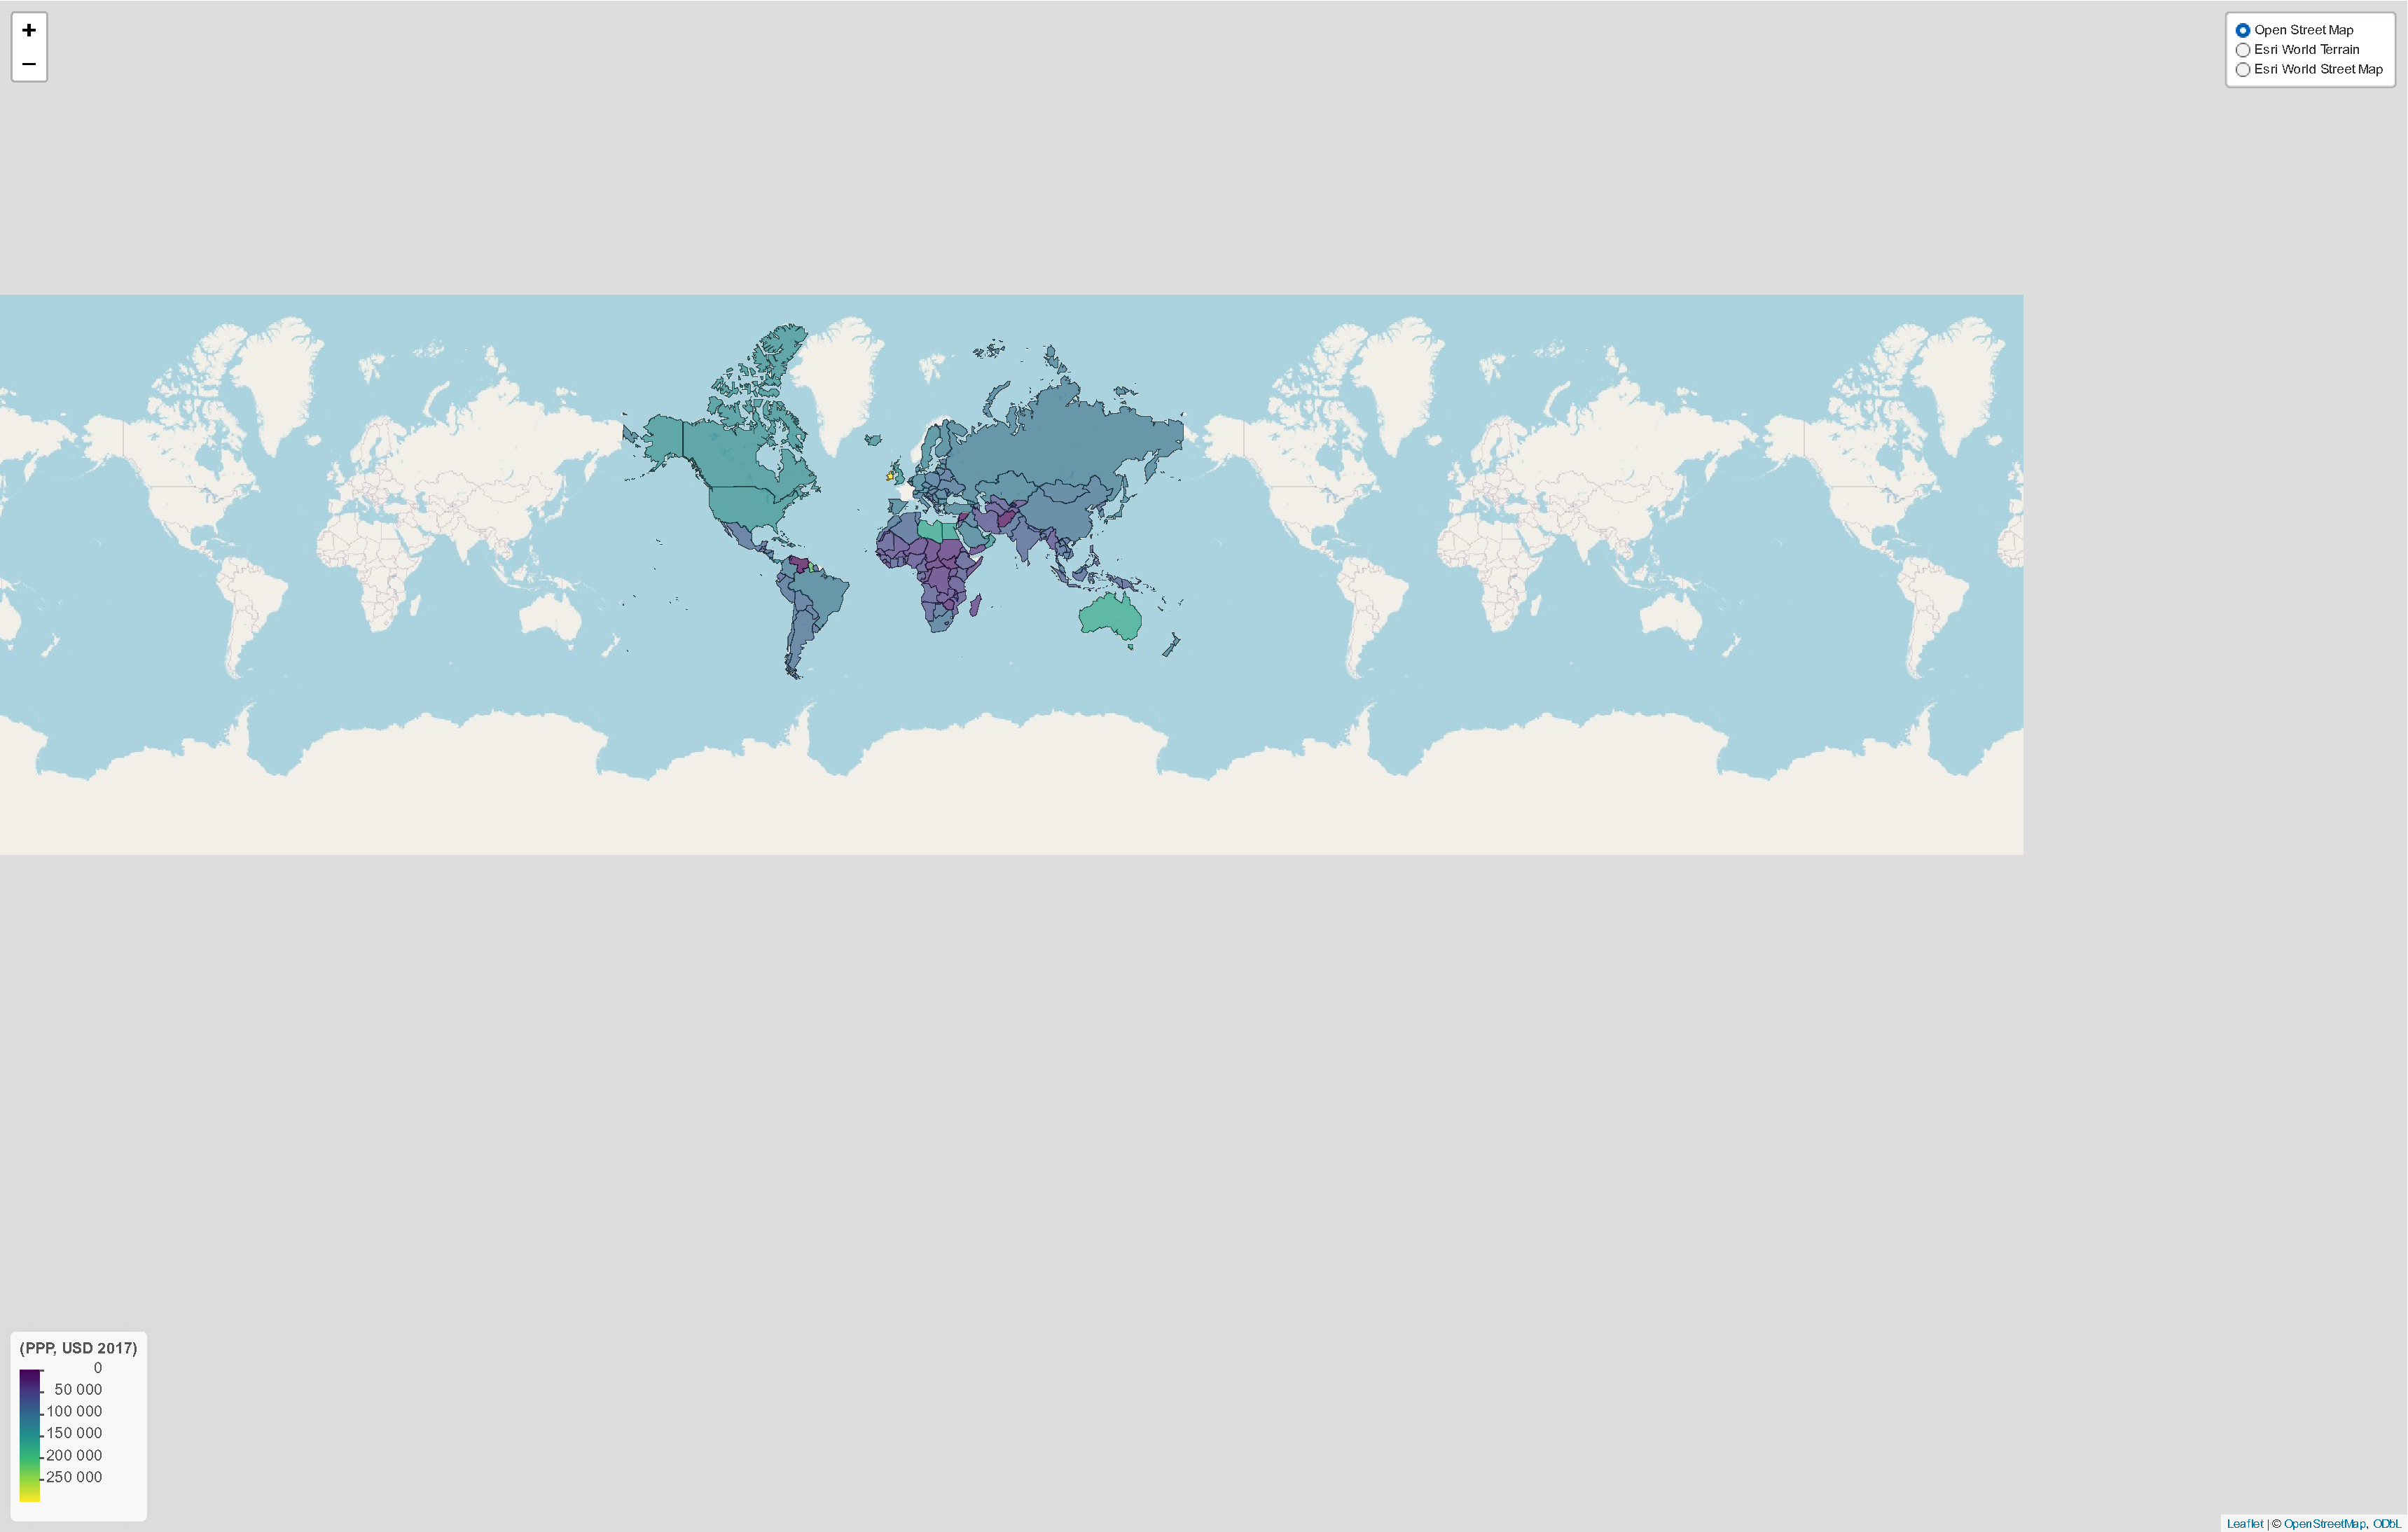
\includegraphics{index_files/figure-pdf/unnamed-chunk-7-1.pdf}

\section{Workflow Overview}\label{workflow-overview}

The standard pipeline involves the steps below. There are
\hyperref[optional-update-input-data]{Optional Steps} to update input
data via API, which are detailed in a separate section. These steps
allow for dynamically retrieving and updating specific datasets before
initiating the pipeline.

\phantomsection\label{workflow-pipeline}
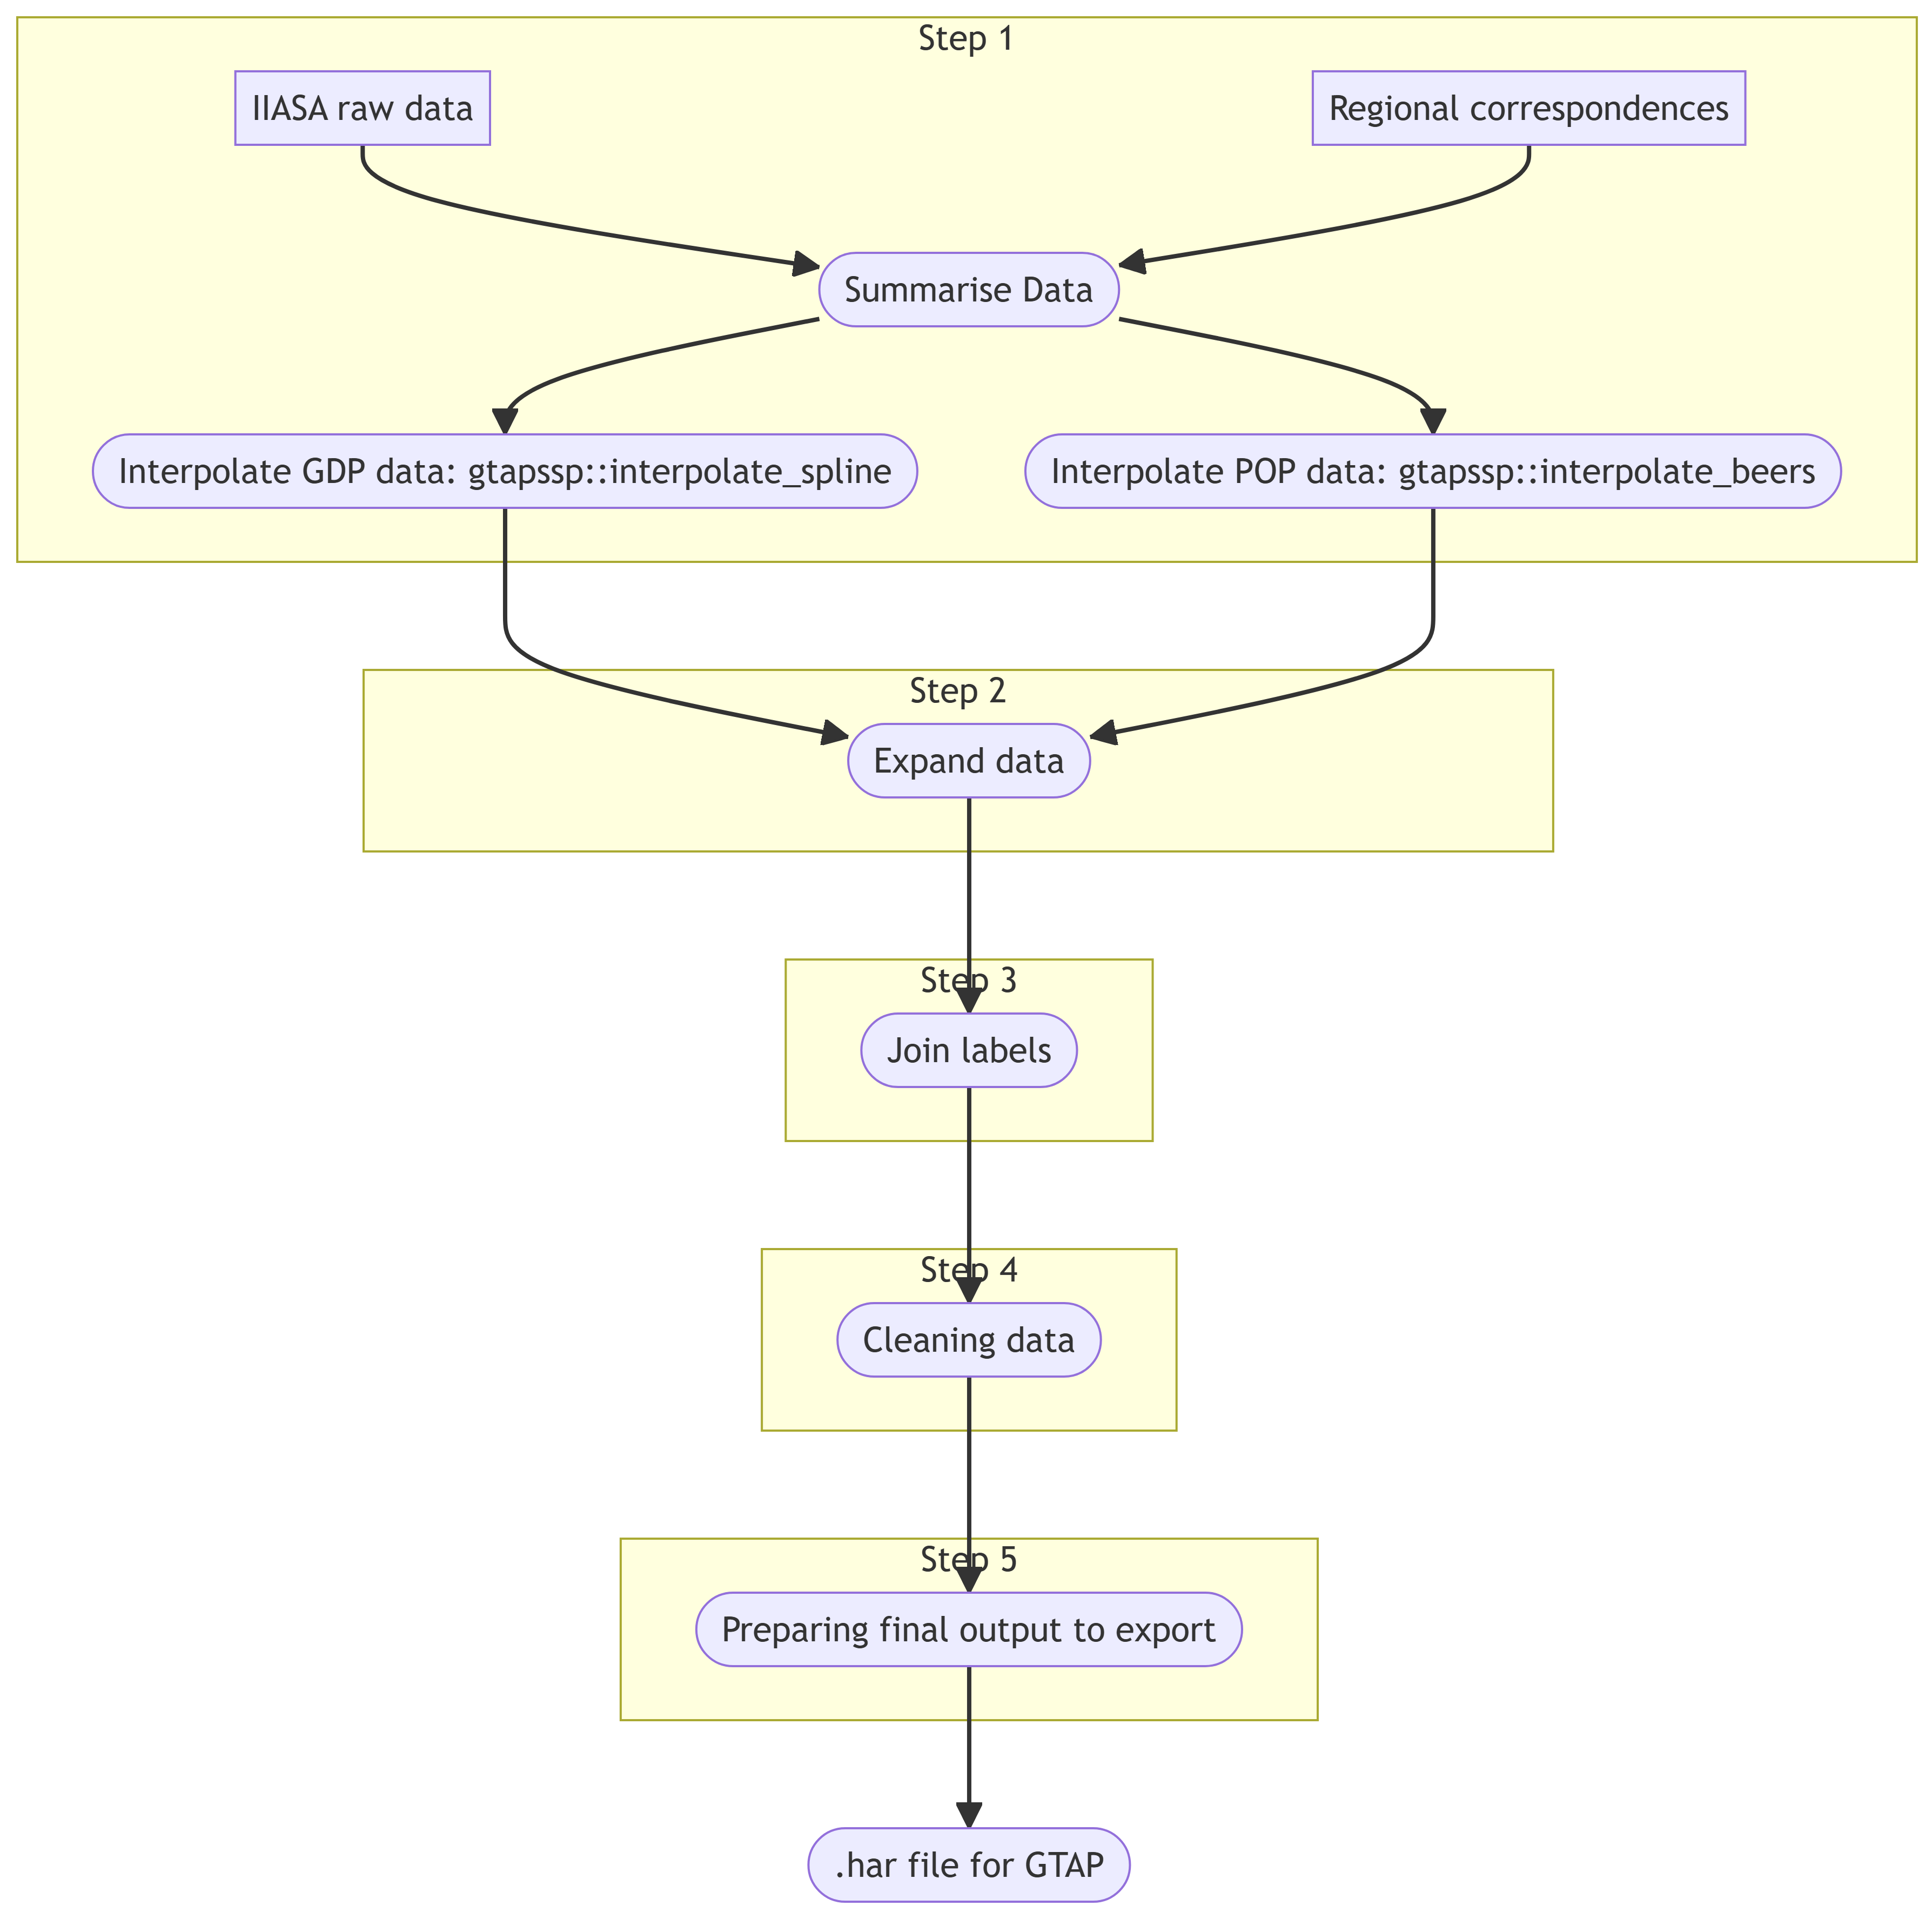
\includegraphics[width=9.32in,height=9.25in]{index_files/figure-latex/mermaid-figure-1.png}

\section{Data Source}\label{data-source}

The pipeline uses projections from the Shared Socioeconomic Pathways
(SSPs) developed by IIASA (version 3.0.1, March 2024). These projections
include \textbf{GDP} and \textbf{Population} data and are publicly
available under a license allowing reuse by other research communities.
For more details, visit the official
\href{https://data.ece.iiasa.ac.at/ssp}{IIASA SSP database}.

Below is a preview of the default IIASA dataset used in the
\texttt{gtapssp} package. This dataset can be updated with the
\texttt{gtapssp::updateData()} function if newer data or custom updates
are required.

\begin{Shaded}
\begin{Highlighting}[]
\NormalTok{gtapssp}\SpecialCharTok{::}\NormalTok{iiasa\_raw}\SpecialCharTok{$}\NormalTok{data}
\end{Highlighting}
\end{Shaded}

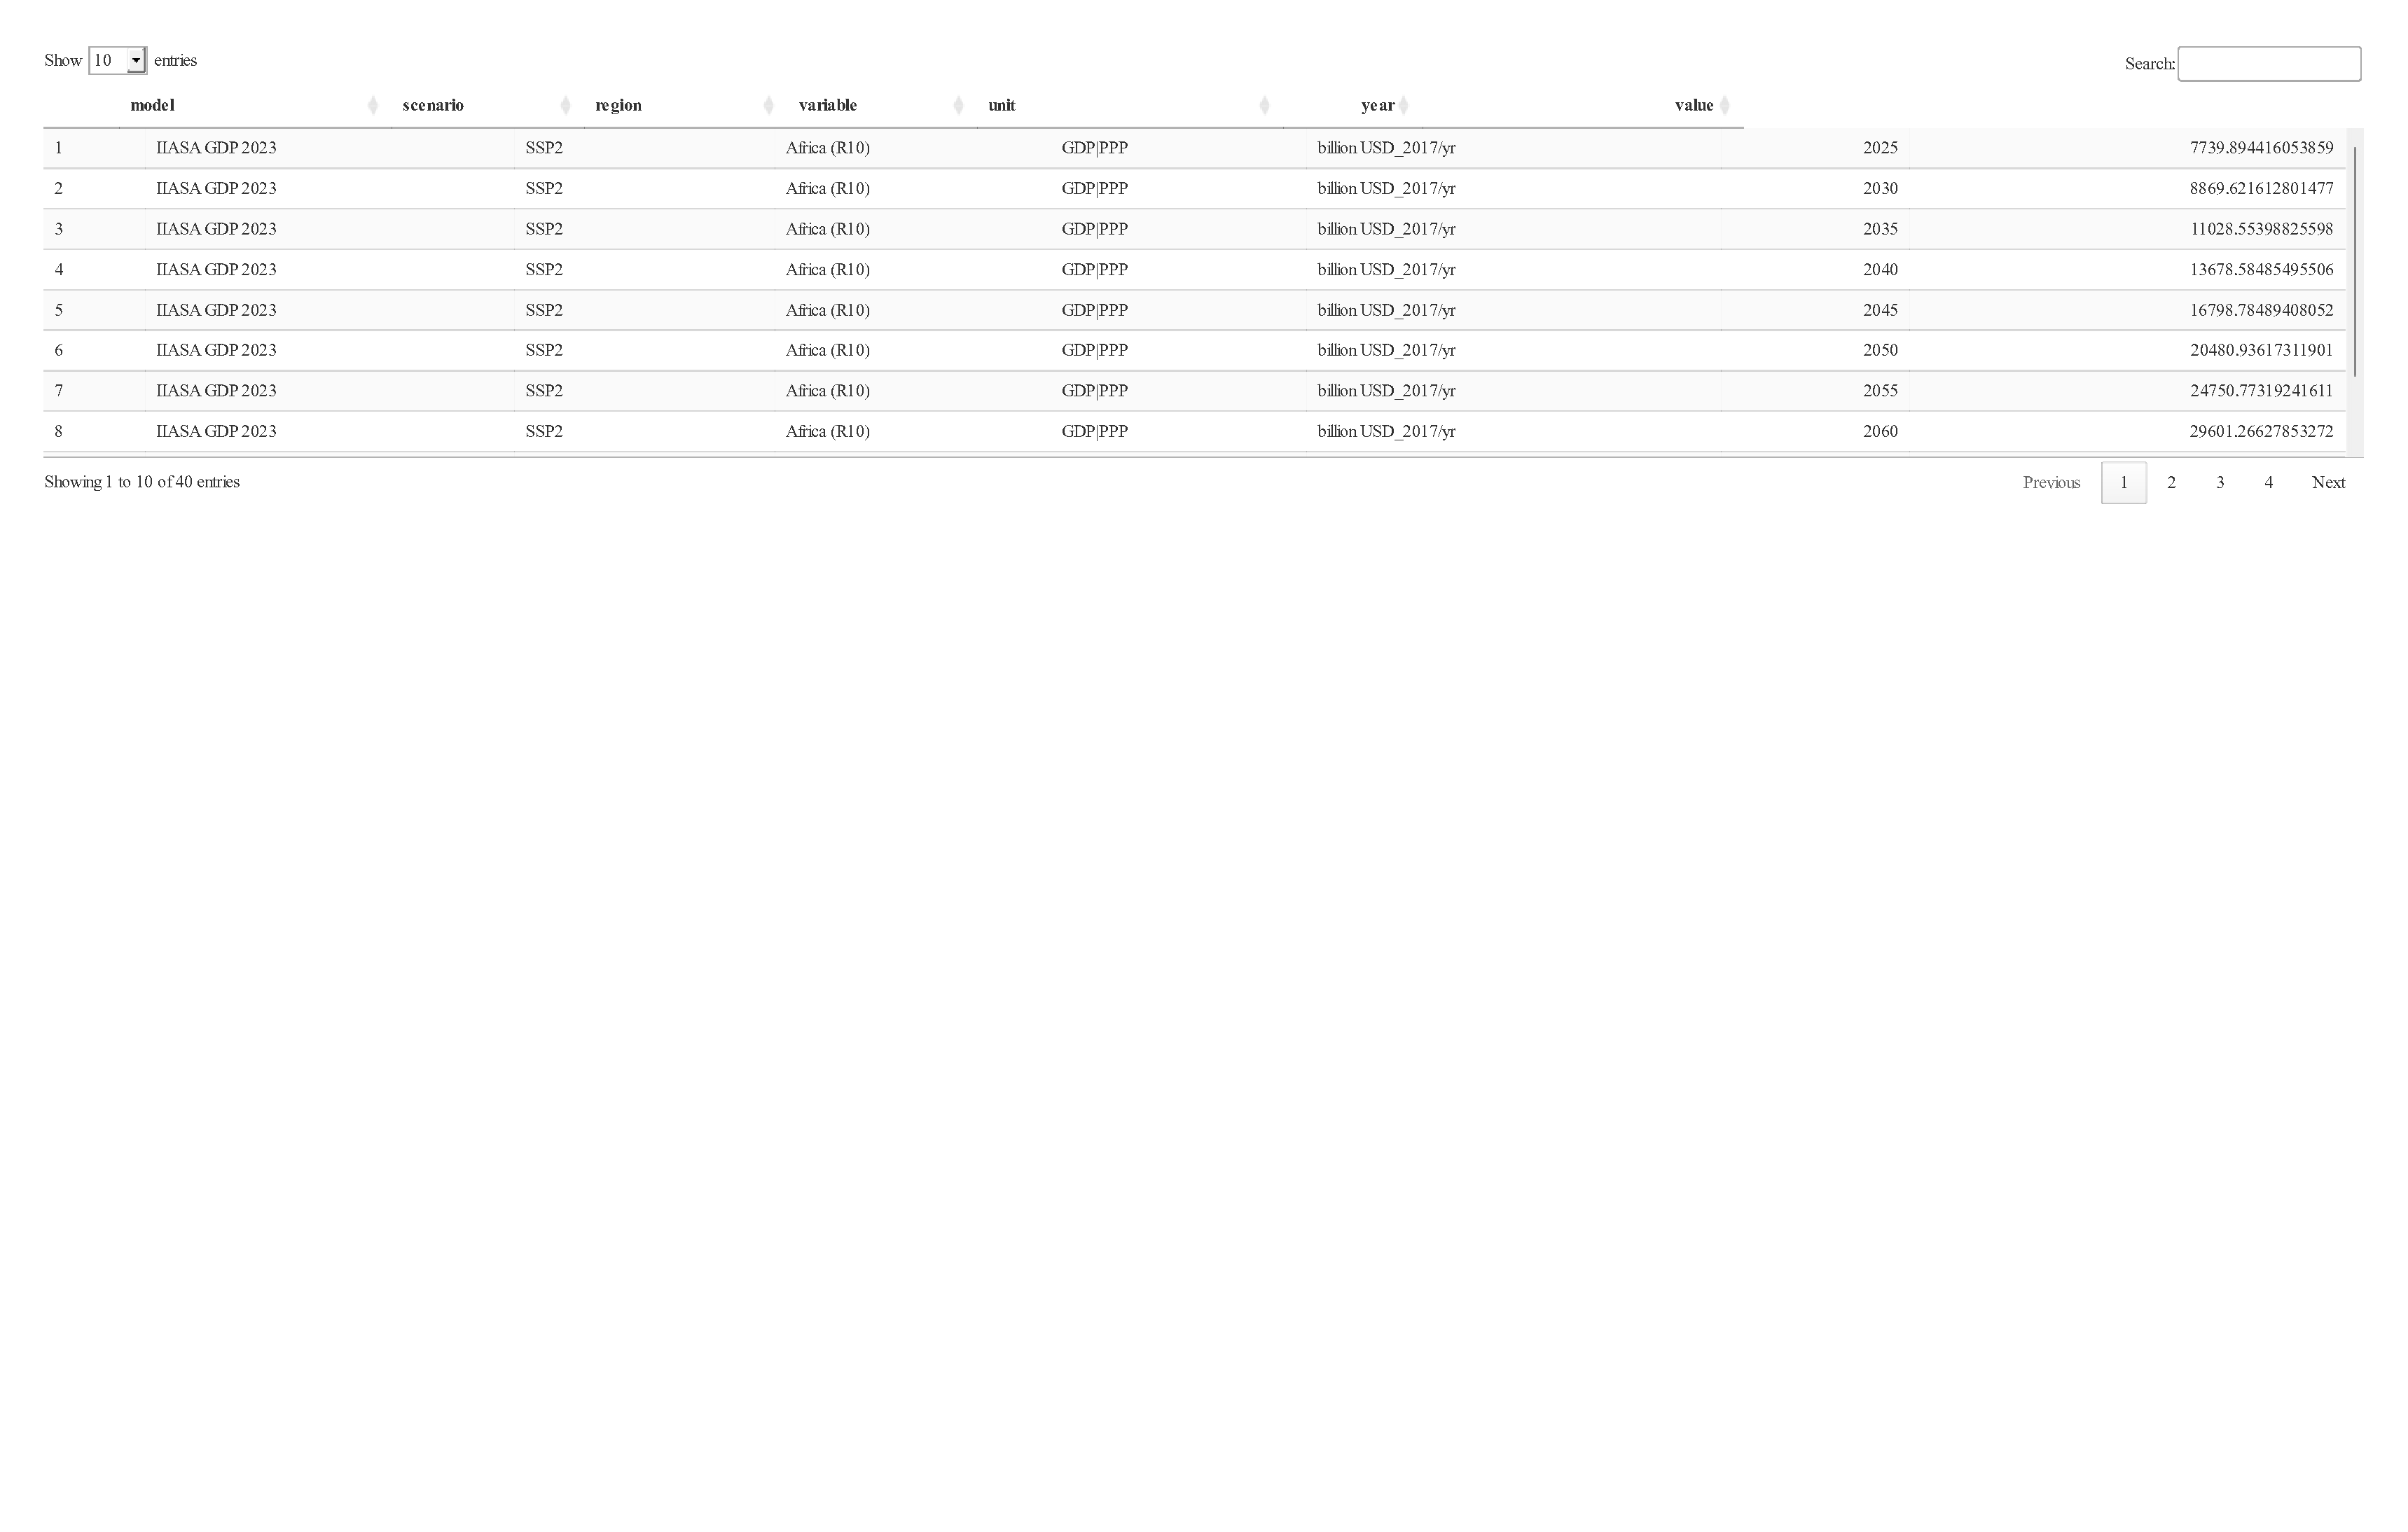
\includegraphics{index_files/figure-pdf/unnamed-chunk-10-1.pdf}

\section{Step 1: Preprocessing and
Aggregation}\label{step-1-preprocessing-and-aggregation}

Aggregate the raw data using \texttt{gtapssp::aggData()}. This function
groups the dataset by specified columns and sums the values within each
group, ensuring compatibility with the GTAP regional structure.

\begin{Shaded}
\begin{Highlighting}[]
\CommentTok{\# Define grouping columns}
\NormalTok{group\_cols }\OtherTok{\textless{}{-}} \FunctionTok{c}\NormalTok{(}\StringTok{"model"}\NormalTok{, }\StringTok{"scenario"}\NormalTok{, }\StringTok{"reg\_iso3"}\NormalTok{, }\StringTok{"variable"}\NormalTok{, }\StringTok{"unit"}\NormalTok{)}
\CommentTok{\# Aggregate raw data}
\NormalTok{agg\_iiasa }\OtherTok{\textless{}{-}}\NormalTok{ gtapssp}\SpecialCharTok{::}\FunctionTok{aggData}\NormalTok{(}
  \AttributeTok{iiasa\_raw =}\NormalTok{ gtapssp}\SpecialCharTok{::}\NormalTok{iiasa\_raw,}
  \AttributeTok{group\_cols =}\NormalTok{ group\_cols}
\NormalTok{)}
\CommentTok{\# Funcion documentation:}
\NormalTok{?gtapssp}\SpecialCharTok{::}\NormalTok{aggData}
\end{Highlighting}
\end{Shaded}

Missing values in the dataset are interpolated using two methods:

\textbf{\texttt{Spline} Interpolation}: Smoothly fills gaps for GDP and
related variables using cubic splines. By default, the function uses the
\texttt{"fmm"} method (default) for interpolation. Users can modify
interpolation parameters for custom behavior. Check the function
documentation for details.

\begin{Shaded}
\begin{Highlighting}[]
\CommentTok{\# Interpolate with spline method}
\NormalTok{spline\_out }\OtherTok{\textless{}{-}}\NormalTok{ agg\_iiasa }\SpecialCharTok{|\textgreater{}}
\NormalTok{  tidyr}\SpecialCharTok{::}\FunctionTok{drop\_na}\NormalTok{(model) }\SpecialCharTok{|\textgreater{}}
\NormalTok{  dplyr}\SpecialCharTok{::}\FunctionTok{filter}\NormalTok{(model }\SpecialCharTok{\%in\%} \FunctionTok{c}\NormalTok{(}\StringTok{"IIASA GDP 2023"}\NormalTok{, }\StringTok{"OECD ENV{-}Growth 2023"}\NormalTok{)) }\SpecialCharTok{|\textgreater{}}
\NormalTok{  gtapssp}\SpecialCharTok{::}\FunctionTok{interpolate\_spline}\NormalTok{(}
    \AttributeTok{groups =}\NormalTok{ group\_cols,}
    \AttributeTok{year =} \StringTok{"year"}\NormalTok{,}
    \AttributeTok{values =} \StringTok{"value"}
\NormalTok{  )}

\CommentTok{\# Funcion documentation:}
\NormalTok{?gtapssp}\SpecialCharTok{::}\NormalTok{interpolate\_spline}
\end{Highlighting}
\end{Shaded}

\textbf{\texttt{Beers} Interpolation}: Specially designed for
demographic data, This function applies the Beers interpolation
algorithm, which is particularly suited for age-cohort data. The default
\texttt{"ordinary"} method preserves population totals while
distributing values evenly across age groups. Additional parameters can
be adjusted as needed; refer to the function documentation for more
information.

\begin{Shaded}
\begin{Highlighting}[]
\CommentTok{\# Interpolate with beers method}
\NormalTok{beers\_out }\OtherTok{\textless{}{-}}\NormalTok{ agg\_iiasa }\SpecialCharTok{|\textgreater{}}
\NormalTok{  dplyr}\SpecialCharTok{::}\FunctionTok{filter}\NormalTok{(model }\SpecialCharTok{\%in\%} \FunctionTok{c}\NormalTok{(}\StringTok{"IIASA{-}WiC POP 2023"}\NormalTok{)) }\SpecialCharTok{|\textgreater{}}
\NormalTok{  dplyr}\SpecialCharTok{::}\FunctionTok{filter}\NormalTok{(}\SpecialCharTok{!}\FunctionTok{grepl}\NormalTok{(}\StringTok{"\^{}Mean Years of Education"}\NormalTok{, variable)) }\SpecialCharTok{|\textgreater{}}
\NormalTok{  gtapssp}\SpecialCharTok{::}\FunctionTok{interpolate\_beers}\NormalTok{(}
    \AttributeTok{groups =}\NormalTok{ group\_cols,}
    \AttributeTok{year =} \StringTok{"year"}\NormalTok{,}
    \AttributeTok{values =} \StringTok{"value"}
\NormalTok{  )}

\CommentTok{\# Split the "variable" column into multiple columns using the delimiter "|".}
\CommentTok{\# This transformation helps to break down the information in "variable" into separate components.}
\CommentTok{\# The new columns will be: "variable", "gender\_code", "cohort", and "education\_level".}

\NormalTok{beers\_out }\OtherTok{\textless{}{-}}\NormalTok{ beers\_out }\SpecialCharTok{|\textgreater{}}
\NormalTok{  tidyr}\SpecialCharTok{::}\FunctionTok{separate\_wider\_delim}\NormalTok{(}
    \AttributeTok{cols =} \StringTok{"variable"}\NormalTok{, }\hspace*{\fill}\NormalTok{\circled{1}}
    \AttributeTok{names =} \FunctionTok{c}\NormalTok{(}\StringTok{"variable"}\NormalTok{, }\StringTok{"gender\_code"}\NormalTok{, }\StringTok{"cohort"}\NormalTok{, }\StringTok{"education\_level"}\NormalTok{), }\hspace*{\fill}\NormalTok{\circled{2}}
    \AttributeTok{delim =} \StringTok{"|"}\NormalTok{, }\hspace*{\fill}\NormalTok{\circled{3}}
    \AttributeTok{too\_few =} \StringTok{"align\_start"} \hspace*{\fill}\NormalTok{\circled{4}}
\NormalTok{  )}

\CommentTok{\# Funcion documentation:}
\NormalTok{?gtapssp}\SpecialCharTok{::}\NormalTok{interpolate\_beers}
\end{Highlighting}
\end{Shaded}

The outputs from the Beers Interpolation (Population data) and Spline
Interpolation (GDP data) are concatenated vertically into a single
dataset.

\begin{Shaded}
\begin{Highlighting}[]
\CommentTok{\# Combine the outputs of GDP and Population data}
\NormalTok{gtap\_ssp }\OtherTok{\textless{}{-}}\NormalTok{ dplyr}\SpecialCharTok{::}\FunctionTok{bind\_rows}\NormalTok{(beers\_out, spline\_out)}
\end{Highlighting}
\end{Shaded}

\section{Step 2: Expanding data}\label{step-2-expanding-data}

The ``Historical Reference'' labels in the \texttt{scenario} dimension
are renamed to match the SSP categories (e.g., SSP1, SSP2, \ldots,
SSP5). This step ensures that the elements in the \texttt{scenario}
dimension are aligned, enabling the creation of a continuous time series
by scenario.

\begin{Shaded}
\begin{Highlighting}[]
\CommentTok{\# Expand scenarios}
\NormalTok{exp\_hist }\OtherTok{\textless{}{-}}\NormalTok{ gtap\_ssp }\SpecialCharTok{|\textgreater{}}
\NormalTok{  dplyr}\SpecialCharTok{::}\FunctionTok{filter}\NormalTok{(scenario }\SpecialCharTok{==} \StringTok{"Historical Reference"}\NormalTok{) }\SpecialCharTok{|\textgreater{}} 
\NormalTok{  dplyr}\SpecialCharTok{::}\FunctionTok{select}\NormalTok{(}\SpecialCharTok{{-}}\NormalTok{scenario) }\SpecialCharTok{|\textgreater{}}                   
\NormalTok{  tidyr}\SpecialCharTok{::}\FunctionTok{expand\_grid}\NormalTok{(}\AttributeTok{scenario =} \FunctionTok{unique}\NormalTok{(gtap\_ssp}\SpecialCharTok{$}\NormalTok{scenario))}

\CommentTok{\# Merge expanded scenarios}
\NormalTok{gtap\_ssp }\OtherTok{\textless{}{-}}\NormalTok{ gtap\_ssp }\SpecialCharTok{|\textgreater{}}
\NormalTok{  dplyr}\SpecialCharTok{::}\FunctionTok{anti\_join}\NormalTok{(dplyr}\SpecialCharTok{::}\FunctionTok{select}\NormalTok{(exp\_hist, }\SpecialCharTok{{-}}\NormalTok{value)) }\SpecialCharTok{|\textgreater{}}
\NormalTok{  dplyr}\SpecialCharTok{::}\FunctionTok{bind\_rows}\NormalTok{(exp\_hist) }\SpecialCharTok{|\textgreater{}}
\NormalTok{  dplyr}\SpecialCharTok{::}\FunctionTok{filter}\NormalTok{(scenario }\SpecialCharTok{!=} \StringTok{"Historical Reference"}\NormalTok{)}
\end{Highlighting}
\end{Shaded}

To ensure completeness to be able to export to a '.har'' file, expand
the dataset to include all combinations of scenarios, regions, and
years.

\begin{Shaded}
\begin{Highlighting}[]
\CommentTok{\# Extract unique combinations of columns excluding \textquotesingle{}scenario\textquotesingle{}, \textquotesingle{}reg\_iso3\textquotesingle{}, \textquotesingle{}year\textquotesingle{}, and \textquotesingle{}value\textquotesingle{}.}
\CommentTok{\# These columns are assumed to represent unique group identifiers for the dataset.}
\NormalTok{unique\_groups }\OtherTok{\textless{}{-}}\NormalTok{ gtap\_ssp }\SpecialCharTok{|\textgreater{}}
\NormalTok{  dplyr}\SpecialCharTok{::}\FunctionTok{select}\NormalTok{(}\SpecialCharTok{{-}}\FunctionTok{c}\NormalTok{(scenario, reg\_iso3, year, value)) }\SpecialCharTok{|\textgreater{}}
\NormalTok{  dplyr}\SpecialCharTok{::}\FunctionTok{distinct}\NormalTok{()  }\CommentTok{\# Retain only distinct rows to define unique group combinations.}

\CommentTok{\# Expand the dataset to include all possible combinations of unique groups with regions, years, and scenarios.}
\NormalTok{complete\_data }\OtherTok{\textless{}{-}}\NormalTok{ unique\_groups }\SpecialCharTok{|\textgreater{}}
\NormalTok{  tidyr}\SpecialCharTok{::}\FunctionTok{expand\_grid}\NormalTok{(}\AttributeTok{reg\_iso3 =} \FunctionTok{unique}\NormalTok{(gtapssp}\SpecialCharTok{::}\NormalTok{corresp\_reg}\SpecialCharTok{$}\NormalTok{reg\_iso3)) }\SpecialCharTok{|\textgreater{}} \CommentTok{\# Add all unique region ISO codes.}
\NormalTok{  tidyr}\SpecialCharTok{::}\FunctionTok{expand\_grid}\NormalTok{(}\AttributeTok{year =} \FunctionTok{unique}\NormalTok{(gtap\_ssp}\SpecialCharTok{$}\NormalTok{year)) }\SpecialCharTok{|\textgreater{}}\CommentTok{\# Add all unique years in the dataset.}
\NormalTok{  tidyr}\SpecialCharTok{::}\FunctionTok{expand\_grid}\NormalTok{(}\AttributeTok{scenario =} \FunctionTok{unique}\NormalTok{(gtap\_ssp}\SpecialCharTok{$}\NormalTok{scenario))}\CommentTok{\# Add all unique SSP scenarios.}

\CommentTok{\# Ensure that all combinations of groups, regions, years, and scenarios exist in the final dataset.}
\CommentTok{\# Any missing combinations will be filled with default values.}
\NormalTok{gtap\_ssp }\OtherTok{\textless{}{-}}\NormalTok{ complete\_data }\SpecialCharTok{|\textgreater{}}
\NormalTok{  dplyr}\SpecialCharTok{::}\FunctionTok{left\_join}\NormalTok{(}
\NormalTok{    gtap\_ssp, }
    \AttributeTok{by =} \FunctionTok{c}\NormalTok{(}\FunctionTok{names}\NormalTok{(unique\_groups), }\StringTok{"scenario"}\NormalTok{, }\StringTok{"reg\_iso3"}\NormalTok{, }\StringTok{"year"}\NormalTok{)  }\CommentTok{\# Merge by all relevant keys.}
\NormalTok{  ) }\SpecialCharTok{|\textgreater{}}
\NormalTok{  dplyr}\SpecialCharTok{::}\FunctionTok{mutate}\NormalTok{(}\AttributeTok{value =}\NormalTok{ tidyr}\SpecialCharTok{::}\FunctionTok{replace\_na}\NormalTok{(value, }\DecValTok{0}\NormalTok{))  }\CommentTok{\# Replace any missing values in the \textquotesingle{}value\textquotesingle{} column with 0.}
\end{Highlighting}
\end{Shaded}

\section{Step 3: Joining labels}\label{step-3-joining-labels}

This step integrates additional labels by merging auxiliary datasets
with the main dataset. It uses ISO codes, educational levels, cohort
categories, and gender information. The default label correspondences
included in the package are shown below. They can be modified with
external sources if needed.

\subsection{Educational Level}

\begin{Shaded}
\begin{Highlighting}[]
\NormalTok{gtapssp}\SpecialCharTok{::}\NormalTok{educDict}
\end{Highlighting}
\end{Shaded}

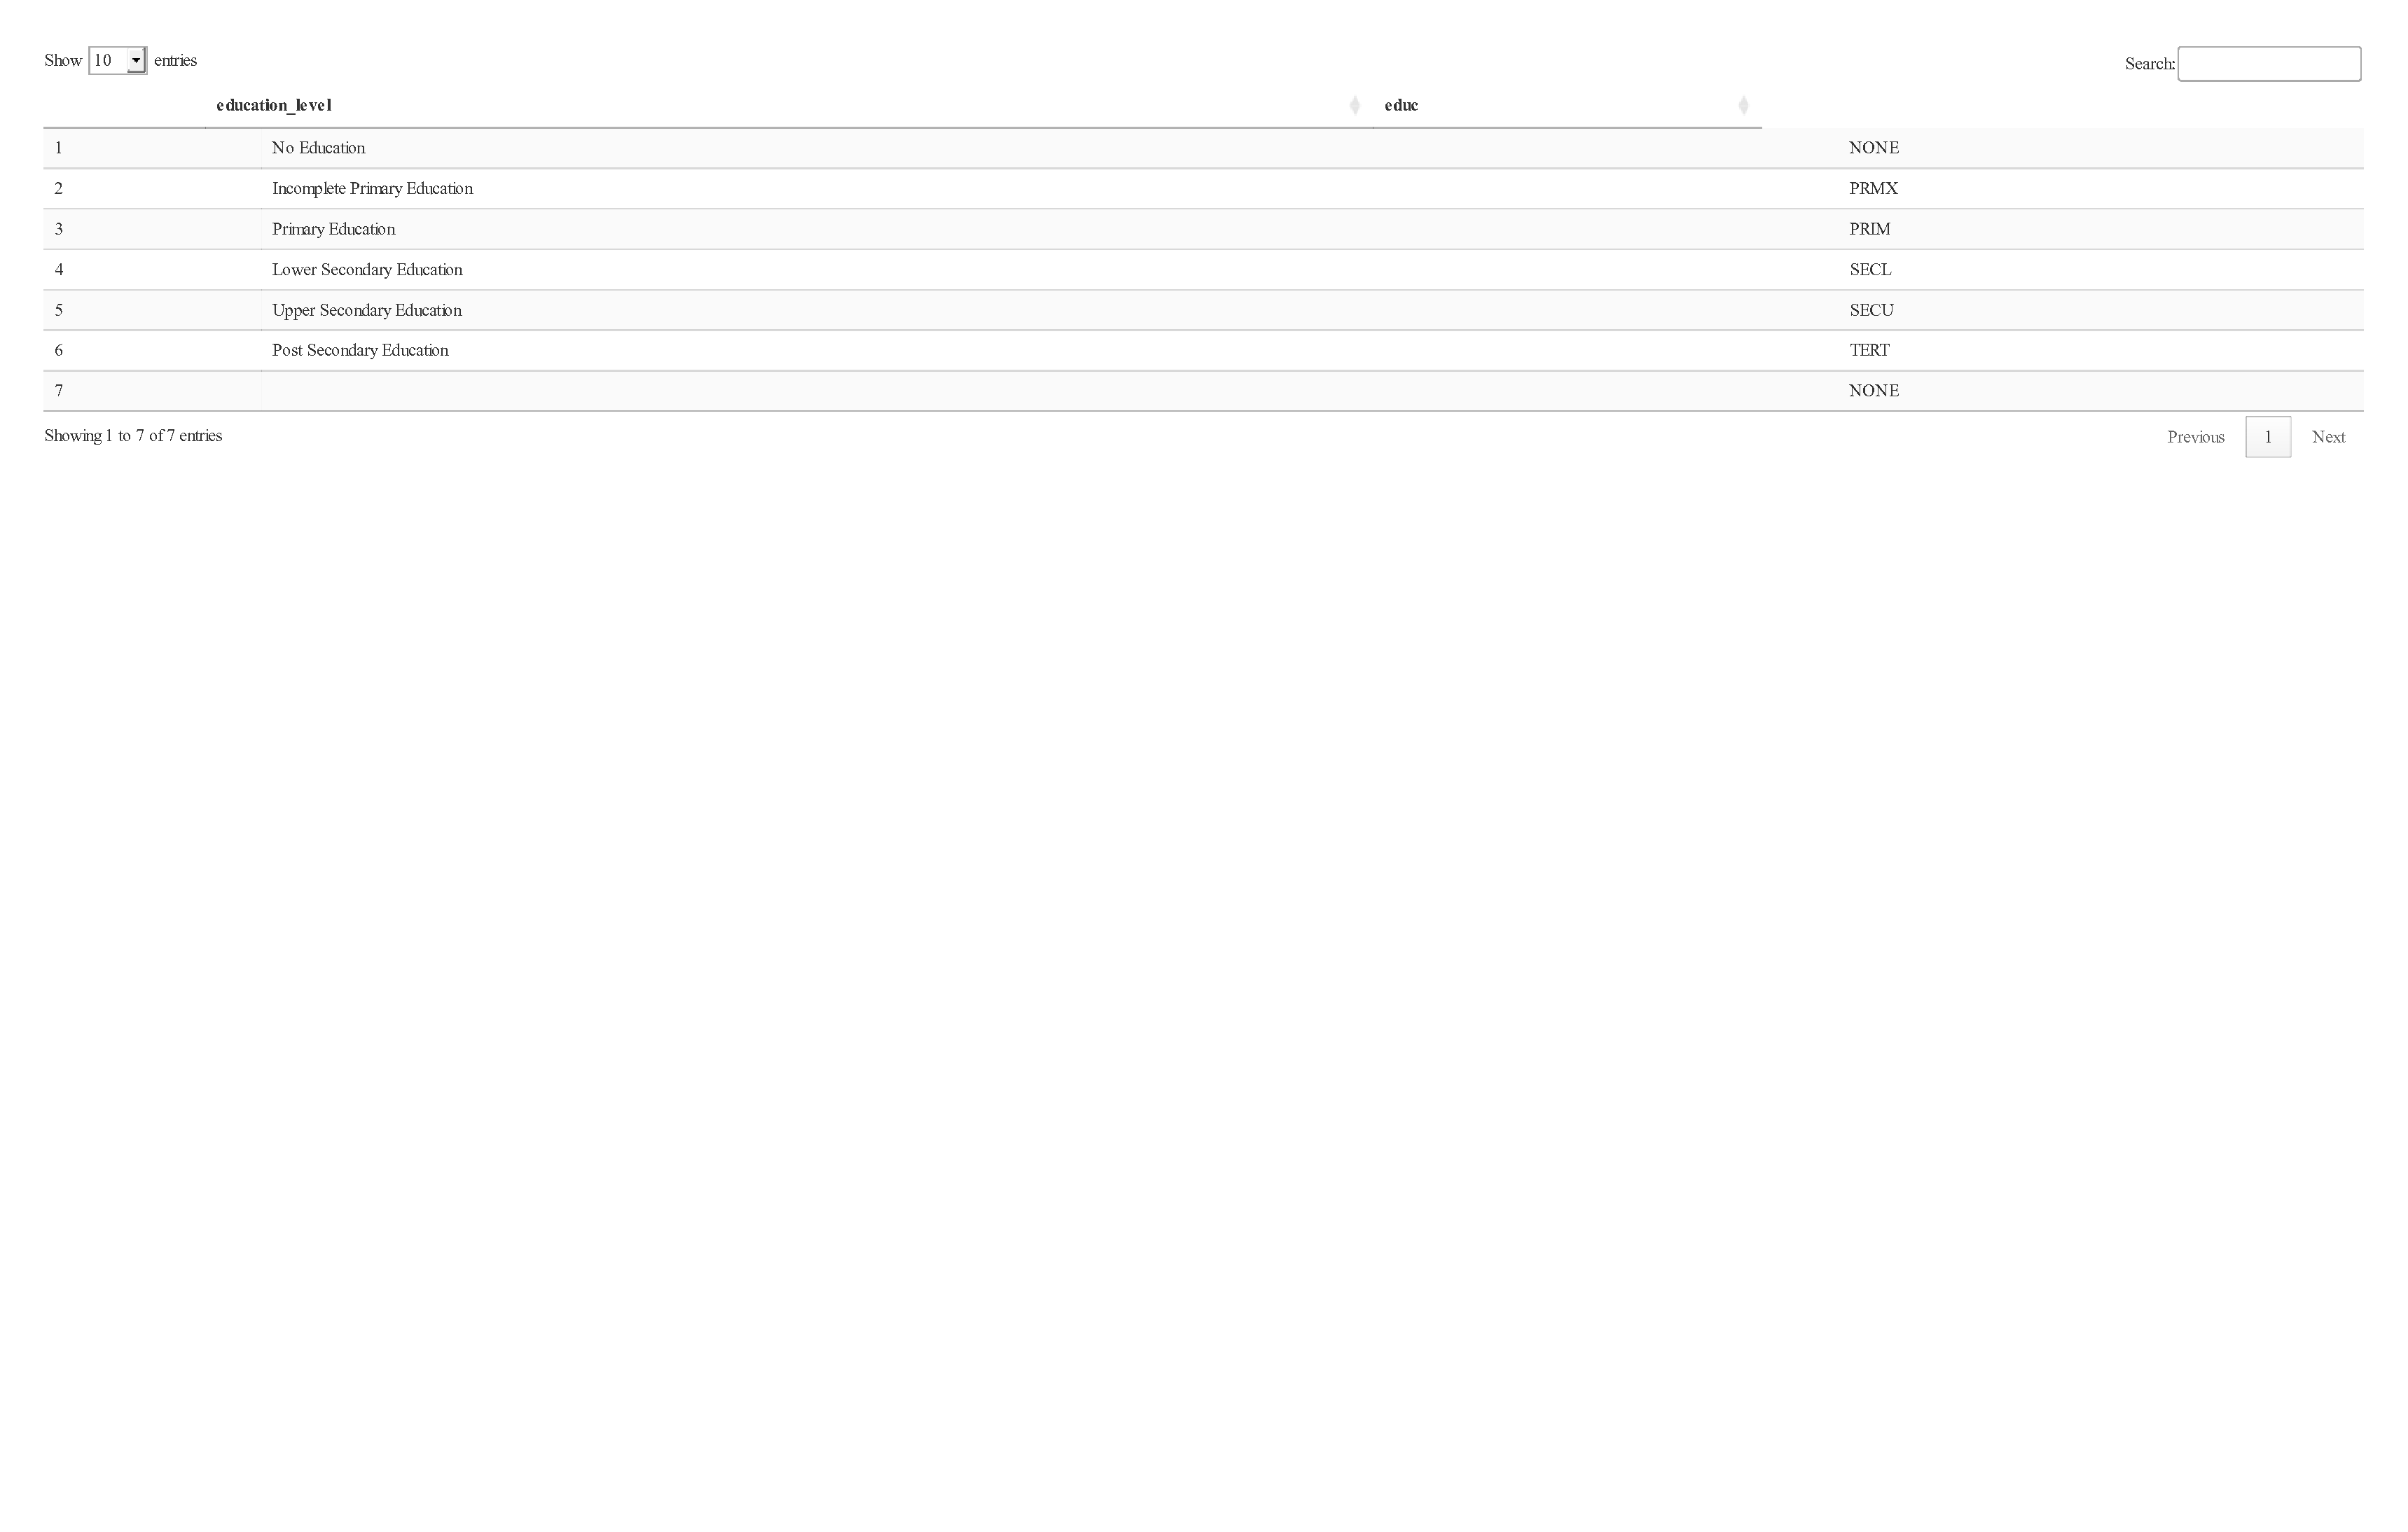
\includegraphics{index_files/figure-pdf/unnamed-chunk-18-1.pdf}

\subsection{Cohort Categories}

\begin{Shaded}
\begin{Highlighting}[]
\NormalTok{gtapssp}\SpecialCharTok{::}\NormalTok{cohortDict}
\end{Highlighting}
\end{Shaded}

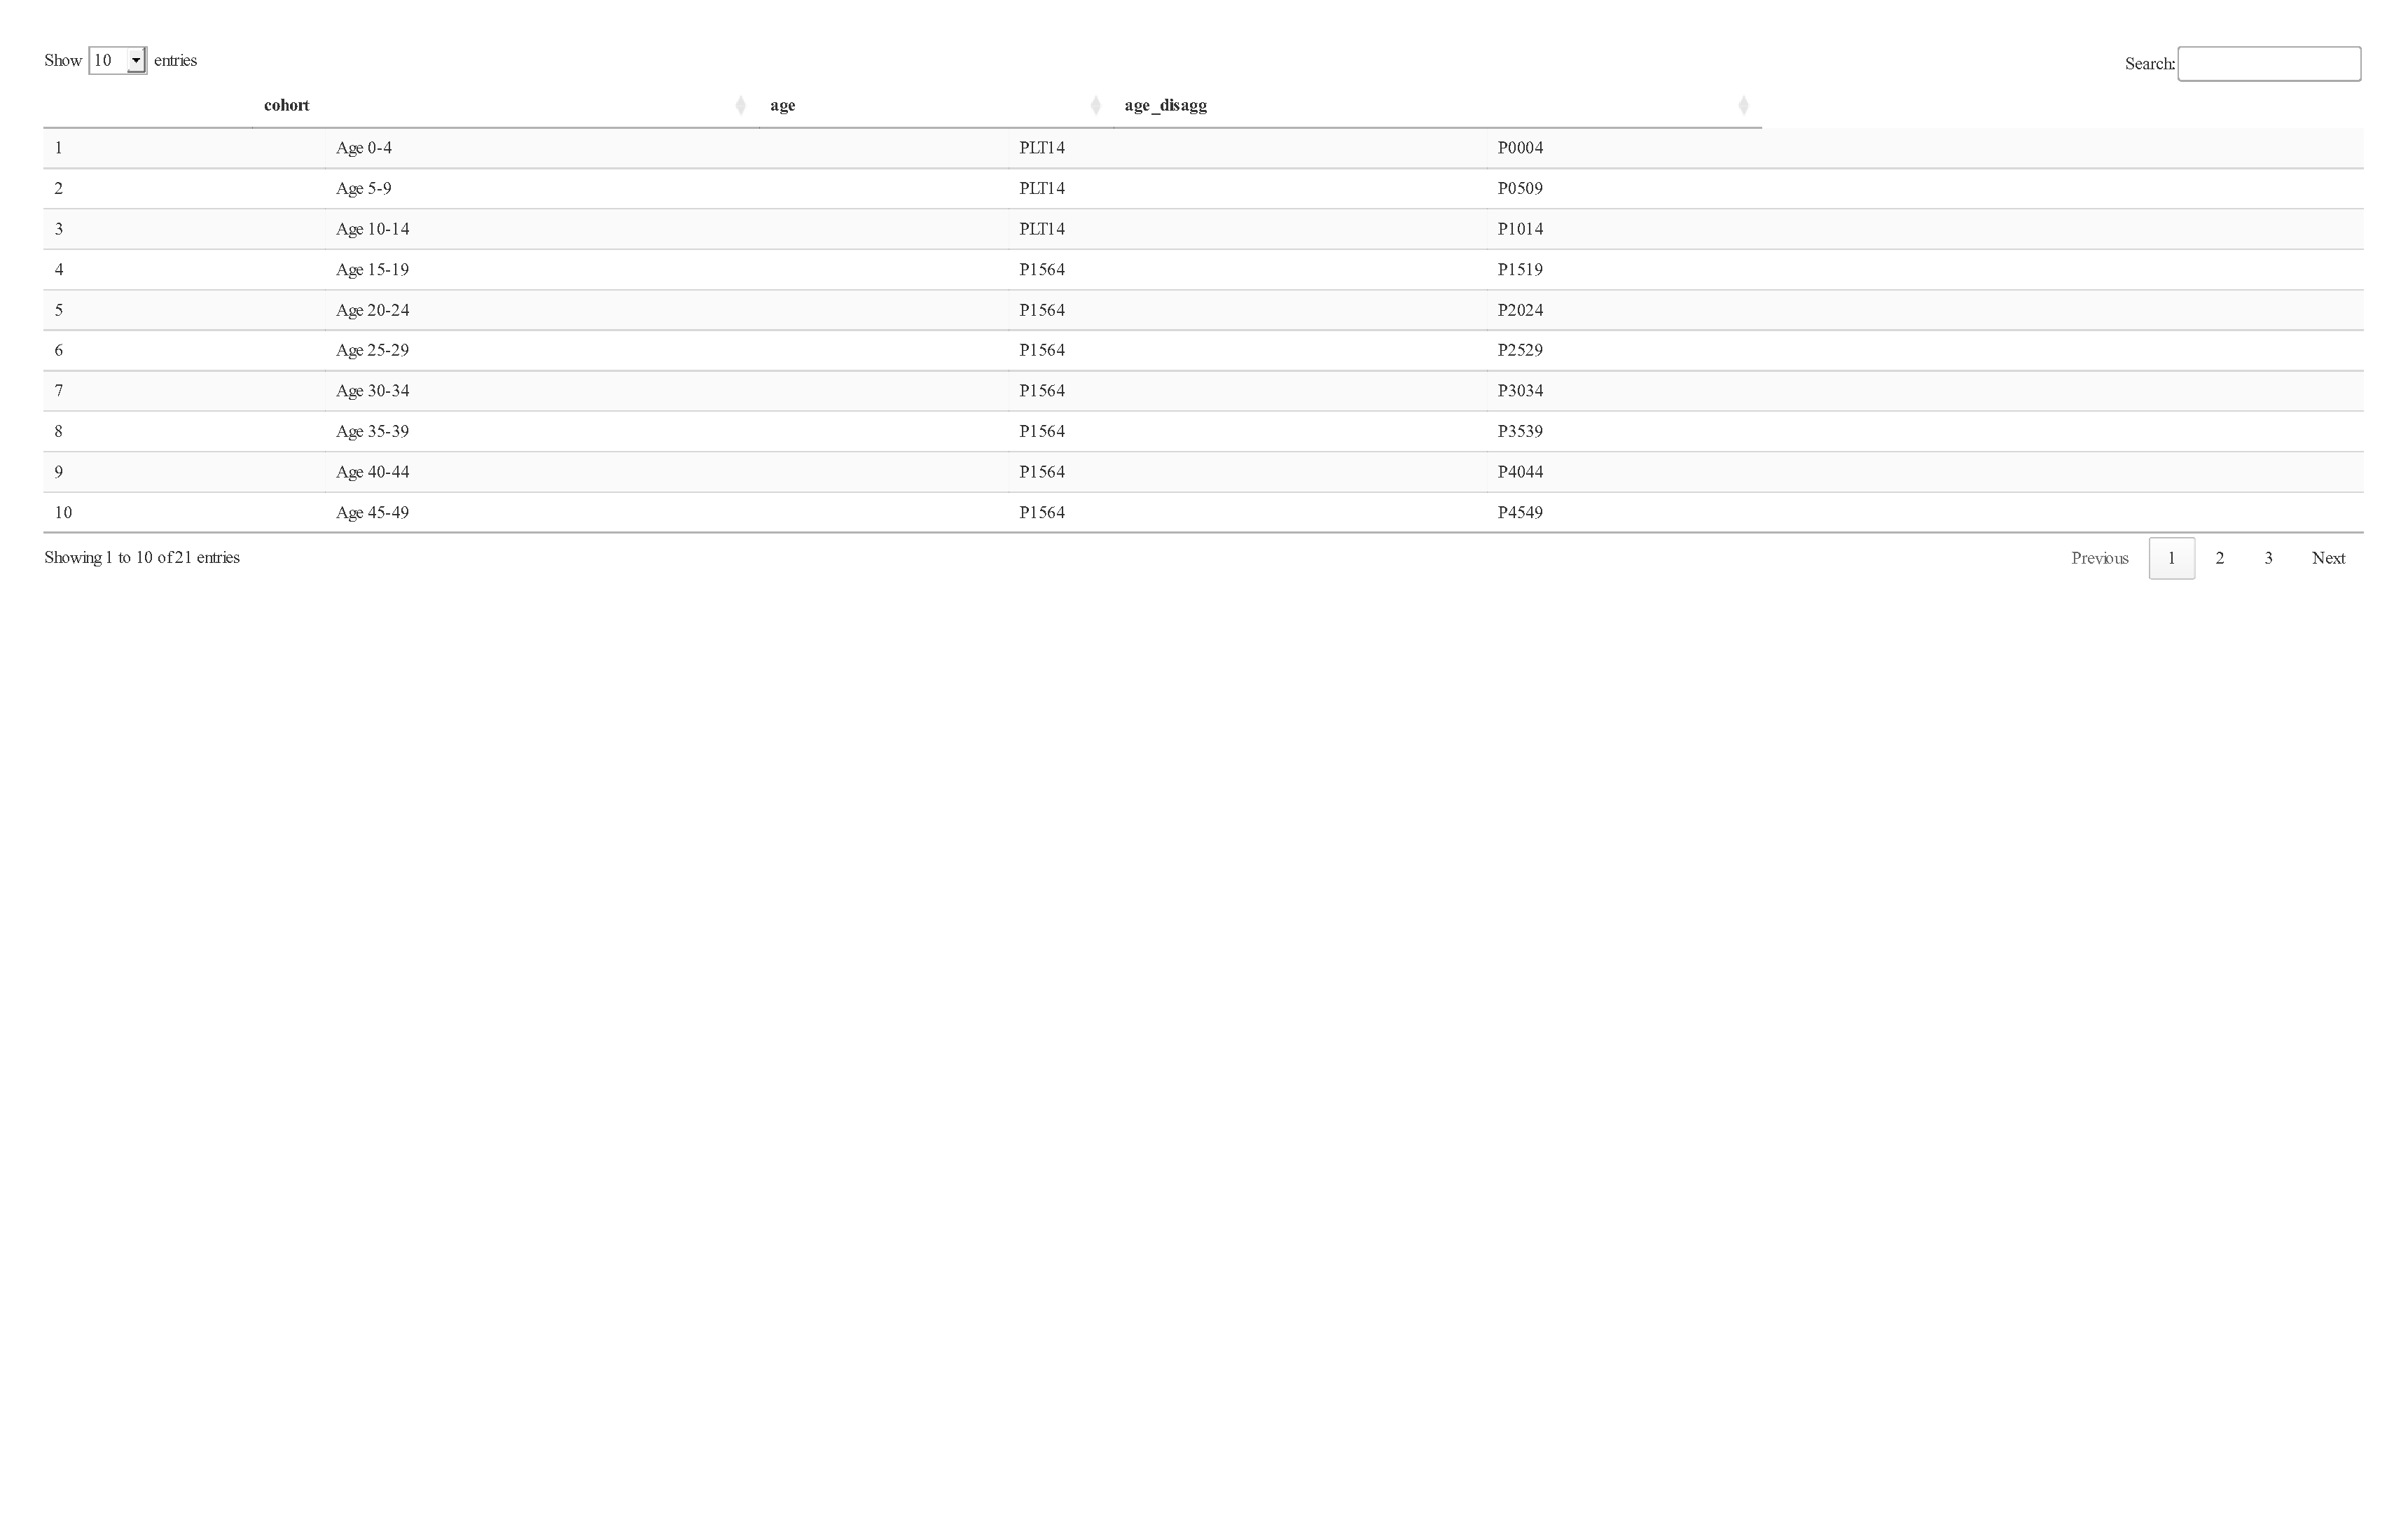
\includegraphics{index_files/figure-pdf/unnamed-chunk-20-1.pdf}

\subsection{Gender Labels}

\begin{Shaded}
\begin{Highlighting}[]
\NormalTok{gtapssp}\SpecialCharTok{::}\NormalTok{genderDict}
\end{Highlighting}
\end{Shaded}

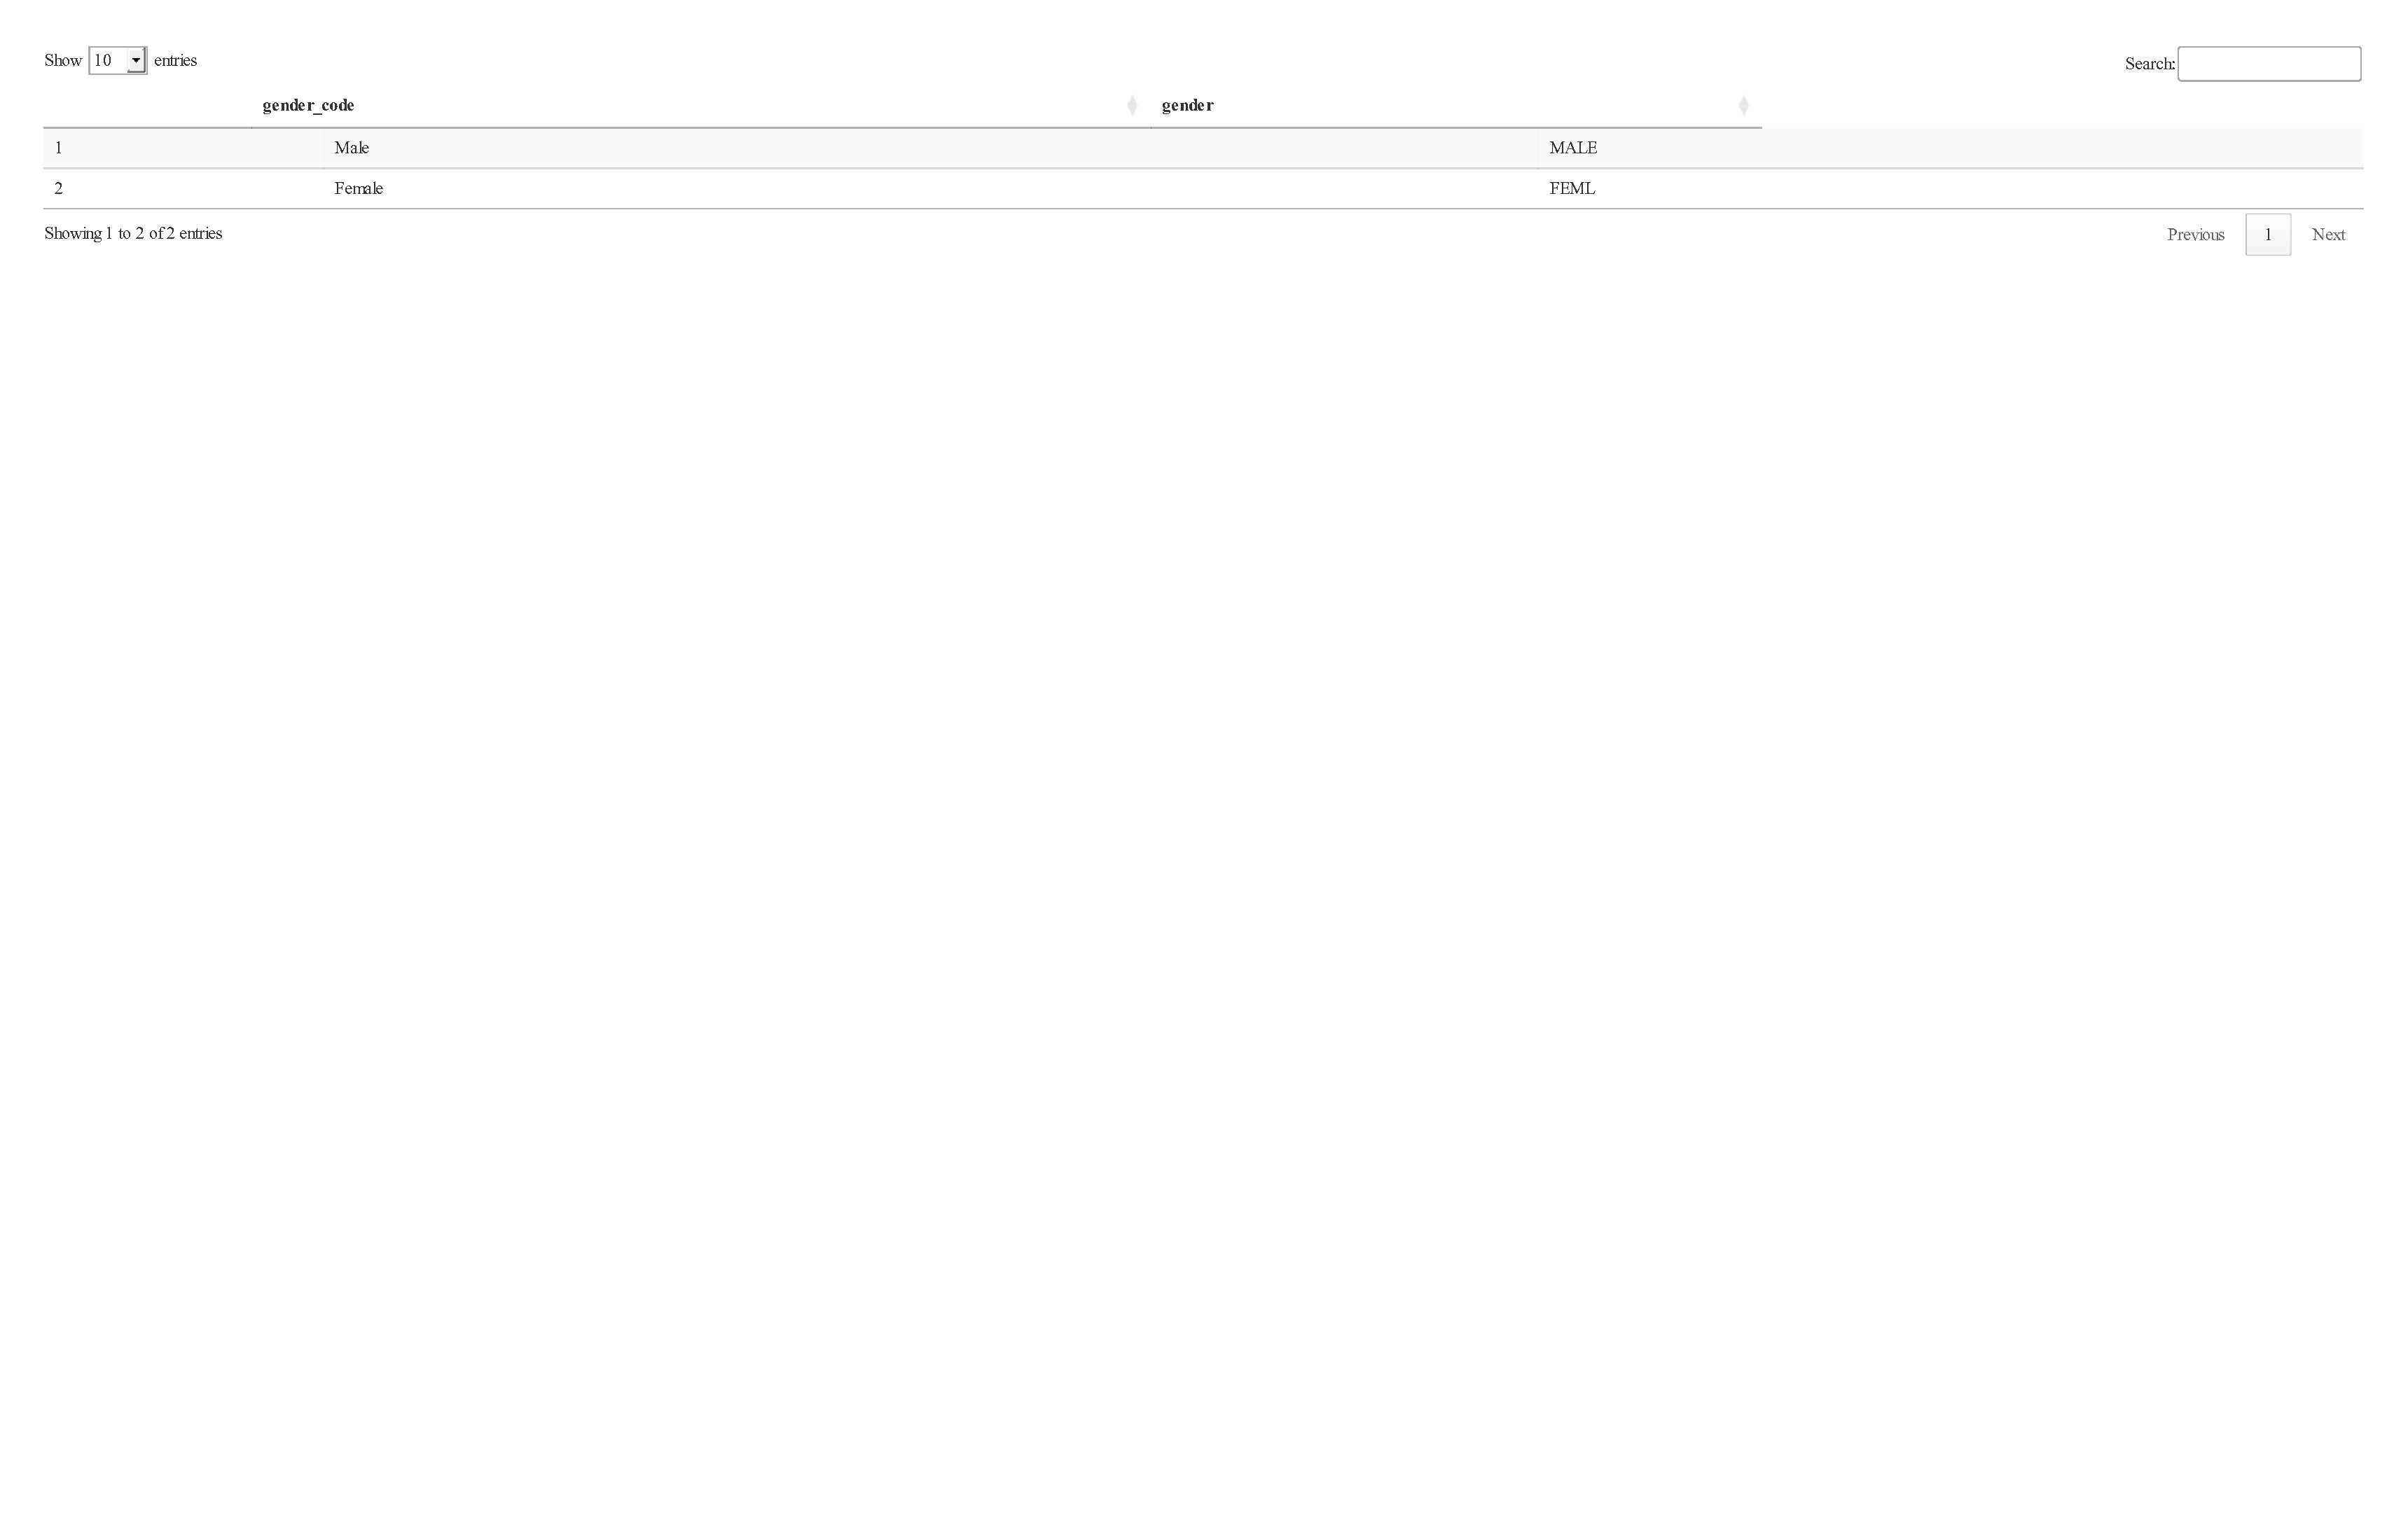
\includegraphics{index_files/figure-pdf/unnamed-chunk-22-1.pdf}

\begin{Shaded}
\begin{Highlighting}[]
\CommentTok{\# Merge the auxiliary datasets with the main dataset (gtap\_ssp)}
\NormalTok{gtap\_ssp }\OtherTok{\textless{}{-}} 
\NormalTok{  gtap\_ssp }\SpecialCharTok{|\textgreater{}}
  \CommentTok{\# Integrate educational level labels}
\NormalTok{  dplyr}\SpecialCharTok{::}\FunctionTok{left\_join}\NormalTok{(gtapssp}\SpecialCharTok{::}\NormalTok{educDict, }\AttributeTok{by =}\NormalTok{ dplyr}\SpecialCharTok{::}\FunctionTok{join\_by}\NormalTok{(education\_level)) }\SpecialCharTok{|\textgreater{}}
  \CommentTok{\# Integrate cohort labels}
\NormalTok{  dplyr}\SpecialCharTok{::}\FunctionTok{left\_join}\NormalTok{(gtapssp}\SpecialCharTok{::}\NormalTok{cohortDict, }\AttributeTok{by =}\NormalTok{ dplyr}\SpecialCharTok{::}\FunctionTok{join\_by}\NormalTok{(cohort)) }\SpecialCharTok{|\textgreater{}}
  \CommentTok{\# Integrate gender labels}
\NormalTok{  dplyr}\SpecialCharTok{::}\FunctionTok{left\_join}\NormalTok{(gtapssp}\SpecialCharTok{::}\NormalTok{genderDict, }\AttributeTok{by =}\NormalTok{ dplyr}\SpecialCharTok{::}\FunctionTok{join\_by}\NormalTok{(gender\_code))}
\end{Highlighting}
\end{Shaded}

\section{Step 4: Cleaning labels}\label{step-4-cleaning-labels}

In this step, the dataset is refined to improve consistency and clarity.
Column names are renamed to standardized 3 characters labels. Missing
values in gender and age are replaced with ``TOTL'' (representing
Total). The variable column for GDP is reclassified, such as converting
``GDP\textbar PPP'' to ``GDP\_PPP.'' Additionally, the values for GDP
(PPP) are adjusted by scaling them by 1000 to reflect the correct units.

\begin{Shaded}
\begin{Highlighting}[]
\NormalTok{gtap\_ssp }\OtherTok{\textless{}{-}} 
\NormalTok{  gtap\_ssp }\SpecialCharTok{|\textgreater{}}
\NormalTok{  dplyr}\SpecialCharTok{::}\FunctionTok{mutate}\NormalTok{(}
    \AttributeTok{MOD =}\NormalTok{ model,                  }\CommentTok{\# Rename \textquotesingle{}model\textquotesingle{} to \textquotesingle{}MOD\textquotesingle{}}
    \AttributeTok{VAR =}\NormalTok{ variable,               }\CommentTok{\# Rename \textquotesingle{}variable\textquotesingle{} to \textquotesingle{}VAR\textquotesingle{}}
    \AttributeTok{SCE =}\NormalTok{ scenario,               }\CommentTok{\# Rename \textquotesingle{}scenario\textquotesingle{} to \textquotesingle{}SCE\textquotesingle{}}
    \AttributeTok{ISO =}\NormalTok{ reg\_iso3,               }\CommentTok{\# Rename \textquotesingle{}reg\_iso3\textquotesingle{} to \textquotesingle{}ISO\textquotesingle{}}
    \AttributeTok{GND =}\NormalTok{ gender,                 }\CommentTok{\# Rename \textquotesingle{}gender\textquotesingle{} to \textquotesingle{}GND\textquotesingle{}}
    \AttributeTok{AGE =}\NormalTok{ age,                    }\CommentTok{\# Rename \textquotesingle{}age\textquotesingle{} to \textquotesingle{}AGE\textquotesingle{}}
    \AttributeTok{YRS =} \FunctionTok{paste0}\NormalTok{(}\StringTok{"Y"}\NormalTok{, year),      }\CommentTok{\# Add "Y" prefix to \textquotesingle{}year\textquotesingle{}}
    \AttributeTok{POP =}\NormalTok{ value,                  }\CommentTok{\# Rename \textquotesingle{}value\textquotesingle{} to \textquotesingle{}POP\textquotesingle{}}
    \AttributeTok{.keep =} \StringTok{"none"}                \CommentTok{\# Keep only the newly defined variables}
\NormalTok{  )}

\NormalTok{gtap\_ssp }\OtherTok{\textless{}{-}} 
\NormalTok{  gtap\_ssp }\SpecialCharTok{|\textgreater{}}
\NormalTok{  dplyr}\SpecialCharTok{::}\FunctionTok{mutate}\NormalTok{(}
    \AttributeTok{GND =}\NormalTok{ tidyr}\SpecialCharTok{::}\FunctionTok{replace\_na}\NormalTok{(GND, }\StringTok{"TOTL"}\NormalTok{), }\CommentTok{\# Replace NA in gender with "TOTL" (Total)}
    \AttributeTok{AGE =}\NormalTok{ tidyr}\SpecialCharTok{::}\FunctionTok{replace\_na}\NormalTok{(AGE, }\StringTok{"TOTL"}\NormalTok{) }\CommentTok{\# Replace NA in age with "TOTL" (Total)}
\NormalTok{  )}

\NormalTok{gtap\_ssp }\OtherTok{\textless{}{-}}\NormalTok{ gtap\_ssp }\SpecialCharTok{|\textgreater{}}
  \CommentTok{\# Modify and transform existing variables using dplyr::mutate}
\NormalTok{  dplyr}\SpecialCharTok{::}\FunctionTok{mutate}\NormalTok{(}
    \CommentTok{\# Reclassify the values of the \textquotesingle{}variable\textquotesingle{} column into a new variable \textquotesingle{}VAR\textquotesingle{}}
    \AttributeTok{VAR =}\NormalTok{ dplyr}\SpecialCharTok{::}\FunctionTok{case\_when}\NormalTok{(}
\NormalTok{      VAR }\SpecialCharTok{==} \StringTok{"GDP|PPP"} \SpecialCharTok{\textasciitilde{}} \StringTok{"GDP\_PPP"}\NormalTok{,                }\CommentTok{\# Replace "GDP|PPP" with "GDP\_PPP"}
\NormalTok{      VAR }\SpecialCharTok{==} \StringTok{"GDP|PPP [per capita]"} \SpecialCharTok{\textasciitilde{}} \StringTok{"GDP\_PER\_CAPI"}\NormalTok{,  }\CommentTok{\# Replace "GDP|PPP [per capita]" with "GDP\_PER\_CAPI"}
      \ConstantTok{TRUE} \SpecialCharTok{\textasciitilde{}}\NormalTok{ VAR                                    }\CommentTok{\# Retain the original values for all other cases}
\NormalTok{    ),}
    \CommentTok{\# Adjust the values in the \textquotesingle{}value\textquotesingle{} column for GDP\_PPP by multiplying by 1000}
    \AttributeTok{POP =} \FunctionTok{ifelse}\NormalTok{(}
\NormalTok{      VAR }\SpecialCharTok{==} \StringTok{"GDP\_PPP"}\NormalTok{,    }\CommentTok{\# Check if the \textquotesingle{}VAR\textquotesingle{} column equals "GDP\_PPP"}
\NormalTok{      POP }\SpecialCharTok{*} \DecValTok{1000}\NormalTok{,        }\CommentTok{\# Multiply the value by 1000 to adjust the unit for absolute values}
\NormalTok{      POP                }\CommentTok{\# Keep the value unchanged for other cases}
\NormalTok{    )}
\NormalTok{  )}

\NormalTok{gtap\_ssp }\OtherTok{\textless{}{-}}\NormalTok{ gtap\_ssp  }\SpecialCharTok{|\textgreater{}}    
\NormalTok{  dplyr}\SpecialCharTok{::}\FunctionTok{filter}\NormalTok{(GND }\SpecialCharTok{!=} \StringTok{"TOTL"} \SpecialCharTok{|}\NormalTok{ MOD }\SpecialCharTok{!=} \StringTok{"IIASA{-}WiC POP 2023"}\NormalTok{) }\SpecialCharTok{|\textgreater{}} \CommentTok{\# Exclude total gender records}
\NormalTok{  dplyr}\SpecialCharTok{::}\FunctionTok{group\_by}\NormalTok{(MOD, VAR, SCE, ISO, GND, YRS, AGE) }\SpecialCharTok{|\textgreater{}} 
\NormalTok{  dplyr}\SpecialCharTok{::}\FunctionTok{summarise}\NormalTok{(}\AttributeTok{value =} \FunctionTok{sum}\NormalTok{(POP, }\AttributeTok{na.rm =}\NormalTok{ T)) }\SpecialCharTok{|\textgreater{}} 
  \FunctionTok{as.data.frame}\NormalTok{()}
\end{Highlighting}
\end{Shaded}

\section{Step 5: Export data}\label{step-5-export-data}

In this step, data is processed into three separate components:
population (\texttt{POP}), GDP projections (\texttt{GDPI}), and GDP from
the OECD ENV-Growth dataset (\texttt{GDPO}). These datasets are then
formatted as arrays and saved to a \texttt{.har} file for further use in
GTAP modeling.

\begin{Shaded}
\begin{Highlighting}[]
\CommentTok{\# Prepare population (POP) dataset}
\NormalTok{POP }\OtherTok{\textless{}{-}}\NormalTok{ gtap\_ssp }\SpecialCharTok{|\textgreater{}}
\NormalTok{   dplyr}\SpecialCharTok{::}\FunctionTok{filter}\NormalTok{(MOD }\SpecialCharTok{==} \StringTok{"IIASA{-}WiC POP 2023"}\NormalTok{) }\SpecialCharTok{|\textgreater{}}               \CommentTok{\# Select population model}
  \CommentTok{\# dplyr::filter(GND != "TOTL") |\textgreater{}                             \# Exclude total gender records}
\NormalTok{  dplyr}\SpecialCharTok{::}\FunctionTok{group\_by}\NormalTok{(SCE, ISO, GND, YRS, AGE) }\SpecialCharTok{|\textgreater{}}                \CommentTok{\# Group by scenario, ISO, gender, year, and age}
\NormalTok{  dplyr}\SpecialCharTok{::}\FunctionTok{summarise}\NormalTok{(}\AttributeTok{POP =} \FunctionTok{sum}\NormalTok{(value, }\AttributeTok{na.rm =}\NormalTok{ T))                 }\CommentTok{\# Sum population values, handling missing data}

\CommentTok{\# Prepare GDP projections (GDPI)}
\NormalTok{GDPI }\OtherTok{\textless{}{-}}\NormalTok{ gtap\_ssp }\SpecialCharTok{|\textgreater{}} 
\NormalTok{  tidyr}\SpecialCharTok{::}\FunctionTok{complete}\NormalTok{(MOD, VAR, SCE, ISO, YRS, }\AttributeTok{fill =} \FunctionTok{list}\NormalTok{(}\AttributeTok{value =} \DecValTok{0}\NormalTok{)) }\SpecialCharTok{|\textgreater{}} \CommentTok{\# Ensure all combinations exist with default values}
\NormalTok{  dplyr}\SpecialCharTok{::}\FunctionTok{filter}\NormalTok{(MOD }\SpecialCharTok{==} \StringTok{"IIASA GDP 2023"}\NormalTok{) }\SpecialCharTok{|\textgreater{}}                         \CommentTok{\# Select IIASA GDP projections model}
\NormalTok{  dplyr}\SpecialCharTok{::}\FunctionTok{filter}\NormalTok{(VAR }\SpecialCharTok{!=} \StringTok{"Population"}\NormalTok{) }\SpecialCharTok{|\textgreater{}}                             \CommentTok{\# Exclude population variables}
\NormalTok{  dplyr}\SpecialCharTok{::}\FunctionTok{group\_by}\NormalTok{(VAR, SCE, ISO, YRS) }\SpecialCharTok{|\textgreater{}}                            \CommentTok{\# Group by variable, scenario, ISO, and year}
\NormalTok{  dplyr}\SpecialCharTok{::}\FunctionTok{summarise}\NormalTok{(}\AttributeTok{GDPI =} \FunctionTok{sum}\NormalTok{(value, }\AttributeTok{na.rm =}\NormalTok{ T))                      }\CommentTok{\# Sum GDP values, handling missing data}

\CommentTok{\# Prepare GDP from OECD ENV{-}Growth dataset (GDPO)}
\NormalTok{GDPO }\OtherTok{\textless{}{-}}\NormalTok{ gtap\_ssp }\SpecialCharTok{|\textgreater{}}
\NormalTok{  dplyr}\SpecialCharTok{::}\FunctionTok{filter}\NormalTok{(MOD }\SpecialCharTok{==} \StringTok{"OECD ENV{-}Growth 2023"}\NormalTok{) }\SpecialCharTok{|\textgreater{}}                  \CommentTok{\# Select GDP from OECD ENV{-}Growth dataset}
\NormalTok{  dplyr}\SpecialCharTok{::}\FunctionTok{group\_by}\NormalTok{(VAR, SCE, ISO, YRS) }\SpecialCharTok{|\textgreater{}}                           \CommentTok{\# Group by variable, scenario, ISO, and year}
\NormalTok{  dplyr}\SpecialCharTok{::}\FunctionTok{summarise}\NormalTok{(}\AttributeTok{GDPO =} \FunctionTok{sum}\NormalTok{(value, }\AttributeTok{na.rm =}\NormalTok{ T))                     }\CommentTok{\# Sum GDP values, handling missing data}
\end{Highlighting}
\end{Shaded}

The processed datasets (\texttt{POP}, \texttt{GDPI}, and \texttt{GDPO})
are converted into arrays, rearranged to 5 dimensions and labeled with
descriptive attributes. These arrays are required for saving into
\texttt{.har} format.

\begin{Shaded}
\begin{Highlighting}[]
\CommentTok{\# Combine datasets into arrays}
\NormalTok{data }\OtherTok{\textless{}{-}} \FunctionTok{list}\NormalTok{(}
  \AttributeTok{POP =} \FunctionTok{array}\NormalTok{(}
\NormalTok{    POP }\SpecialCharTok{|\textgreater{}}\NormalTok{ dplyr}\SpecialCharTok{::}\FunctionTok{pull}\NormalTok{(POP),                                      }\CommentTok{\# Extract population values}
    \AttributeTok{dim =} \FunctionTok{rev}\NormalTok{(}\FunctionTok{sapply}\NormalTok{(POP }\SpecialCharTok{|\textgreater{}}\NormalTok{ dplyr}\SpecialCharTok{::}\FunctionTok{select}\NormalTok{(}\SpecialCharTok{{-}}\NormalTok{POP), }\ControlFlowTok{function}\NormalTok{(x) }\FunctionTok{length}\NormalTok{(}\FunctionTok{unique}\NormalTok{(x)))), }\CommentTok{\# Define dimensions}
    \AttributeTok{dimnames =} \FunctionTok{rev}\NormalTok{(}\FunctionTok{lapply}\NormalTok{(POP }\SpecialCharTok{|\textgreater{}}\NormalTok{ dplyr}\SpecialCharTok{::}\FunctionTok{select}\NormalTok{(}\SpecialCharTok{{-}}\NormalTok{POP), }\ControlFlowTok{function}\NormalTok{(x) }\FunctionTok{unique}\NormalTok{(x)))     }\CommentTok{\# Define dimension names}
\NormalTok{  ) }\SpecialCharTok{|\textgreater{}} \FunctionTok{aperm}\NormalTok{(}\FunctionTok{rev}\NormalTok{(}\DecValTok{1}\SpecialCharTok{:}\NormalTok{(}\FunctionTok{length}\NormalTok{(POP) }\SpecialCharTok{{-}} \DecValTok{1}\NormalTok{))),                           }\CommentTok{\# Adjust dimension order}
  
  \AttributeTok{GDPI =} \FunctionTok{array}\NormalTok{(}
\NormalTok{    GDPI }\SpecialCharTok{|\textgreater{}}\NormalTok{ dplyr}\SpecialCharTok{::}\FunctionTok{pull}\NormalTok{(GDPI),                                    }\CommentTok{\# Extract GDP values (IIASA)}
    \AttributeTok{dim =} \FunctionTok{rev}\NormalTok{(}\FunctionTok{sapply}\NormalTok{(GDPI }\SpecialCharTok{|\textgreater{}}\NormalTok{ dplyr}\SpecialCharTok{::}\FunctionTok{select}\NormalTok{(}\SpecialCharTok{{-}}\NormalTok{GDPI), }\ControlFlowTok{function}\NormalTok{(x) }\FunctionTok{length}\NormalTok{(}\FunctionTok{unique}\NormalTok{(x)))), }\CommentTok{\# Define dimensions}
    \AttributeTok{dimnames =} \FunctionTok{rev}\NormalTok{(}\FunctionTok{lapply}\NormalTok{(GDPI }\SpecialCharTok{|\textgreater{}}\NormalTok{ dplyr}\SpecialCharTok{::}\FunctionTok{select}\NormalTok{(}\SpecialCharTok{{-}}\NormalTok{GDPI), }\ControlFlowTok{function}\NormalTok{(x) }\FunctionTok{unique}\NormalTok{(x)))     }\CommentTok{\# Define dimension names}
\NormalTok{  ) }\SpecialCharTok{|\textgreater{}} \FunctionTok{aperm}\NormalTok{(}\FunctionTok{rev}\NormalTok{(}\DecValTok{1}\SpecialCharTok{:}\NormalTok{(}\FunctionTok{length}\NormalTok{(GDPI) }\SpecialCharTok{{-}} \DecValTok{1}\NormalTok{))),                          }\CommentTok{\# Adjust dimension order}
  
  \AttributeTok{GDPO =} \FunctionTok{array}\NormalTok{(}
\NormalTok{    GDPO }\SpecialCharTok{|\textgreater{}}\NormalTok{ dplyr}\SpecialCharTok{::}\FunctionTok{pull}\NormalTok{(GDPO),                                    }\CommentTok{\# Extract GDP values (OECD)}
    \AttributeTok{dim =} \FunctionTok{rev}\NormalTok{(}\FunctionTok{sapply}\NormalTok{(GDPO }\SpecialCharTok{|\textgreater{}}\NormalTok{ dplyr}\SpecialCharTok{::}\FunctionTok{select}\NormalTok{(}\SpecialCharTok{{-}}\NormalTok{GDPO), }\ControlFlowTok{function}\NormalTok{(x) }\FunctionTok{length}\NormalTok{(}\FunctionTok{unique}\NormalTok{(x)))), }\CommentTok{\# Define dimensions}
    \AttributeTok{dimnames =} \FunctionTok{rev}\NormalTok{(}\FunctionTok{lapply}\NormalTok{(GDPO }\SpecialCharTok{|\textgreater{}}\NormalTok{ dplyr}\SpecialCharTok{::}\FunctionTok{select}\NormalTok{(}\SpecialCharTok{{-}}\NormalTok{GDPO), }\ControlFlowTok{function}\NormalTok{(x) }\FunctionTok{unique}\NormalTok{(x)))     }\CommentTok{\# Define dimension names}
\NormalTok{  ) }\SpecialCharTok{|\textgreater{}} \FunctionTok{aperm}\NormalTok{(}\FunctionTok{rev}\NormalTok{(}\DecValTok{1}\SpecialCharTok{:}\NormalTok{(}\FunctionTok{length}\NormalTok{(GDPO) }\SpecialCharTok{{-}} \DecValTok{1}\NormalTok{)))                           }\CommentTok{\# Adjust dimension order}
\NormalTok{)}

\CommentTok{\# Add descriptive metadata to arrays}
\FunctionTok{attr}\NormalTok{(data}\SpecialCharTok{$}\NormalTok{POP, }\StringTok{"description"}\NormalTok{) }\OtherTok{\textless{}{-}} \StringTok{"IIASA{-}WiC POP 2023 (million people)"}       \CommentTok{\# Population description}
\FunctionTok{attr}\NormalTok{(data}\SpecialCharTok{$}\NormalTok{GDPI, }\StringTok{"description"}\NormalTok{) }\OtherTok{\textless{}{-}} \StringTok{"IIASA GDP 2023 (USD\_2017/yr)"}             \CommentTok{\# GDP projections description}
\FunctionTok{attr}\NormalTok{(data}\SpecialCharTok{$}\NormalTok{GDPO, }\StringTok{"description"}\NormalTok{) }\OtherTok{\textless{}{-}} \StringTok{"OECD ENV{-}Growth 2023 (USD\_2017/yr)"}       \CommentTok{\# OECD GDP description}
\end{Highlighting}
\end{Shaded}

Save the prepared data arrays into a \texttt{.har} file using the
\texttt{HARr::write\_har} function.

\begin{Shaded}
\begin{Highlighting}[]
\CommentTok{\# Export datasets to a .har file}
\NormalTok{HARr}\SpecialCharTok{::}\FunctionTok{write\_har}\NormalTok{(data, }\StringTok{"gtap\_ssp.har"}\NormalTok{)}
\end{Highlighting}
\end{Shaded}

\section{Optional: Update input data}\label{optional-update-input-data}

The gtapssp::updateData() function allows users to download and process
the latest version of the SSPs dataset from the IIASA database. This
step is optional and should be used if you want to replace the default
SSP dataset included in the gtapssp package (gtapssp::iiasa\_raw) with a
newer version. The updated data is processed using Python's pyam package
and may take several minutes depending on the database size. For more
details on the pyam package and its integration with R, visit
\href{https://pyam-iamc.readthedocs.io/en/stable/R_tutorials/pyam_R_tutorial.html}{here}.

\phantomsection\label{optinional}
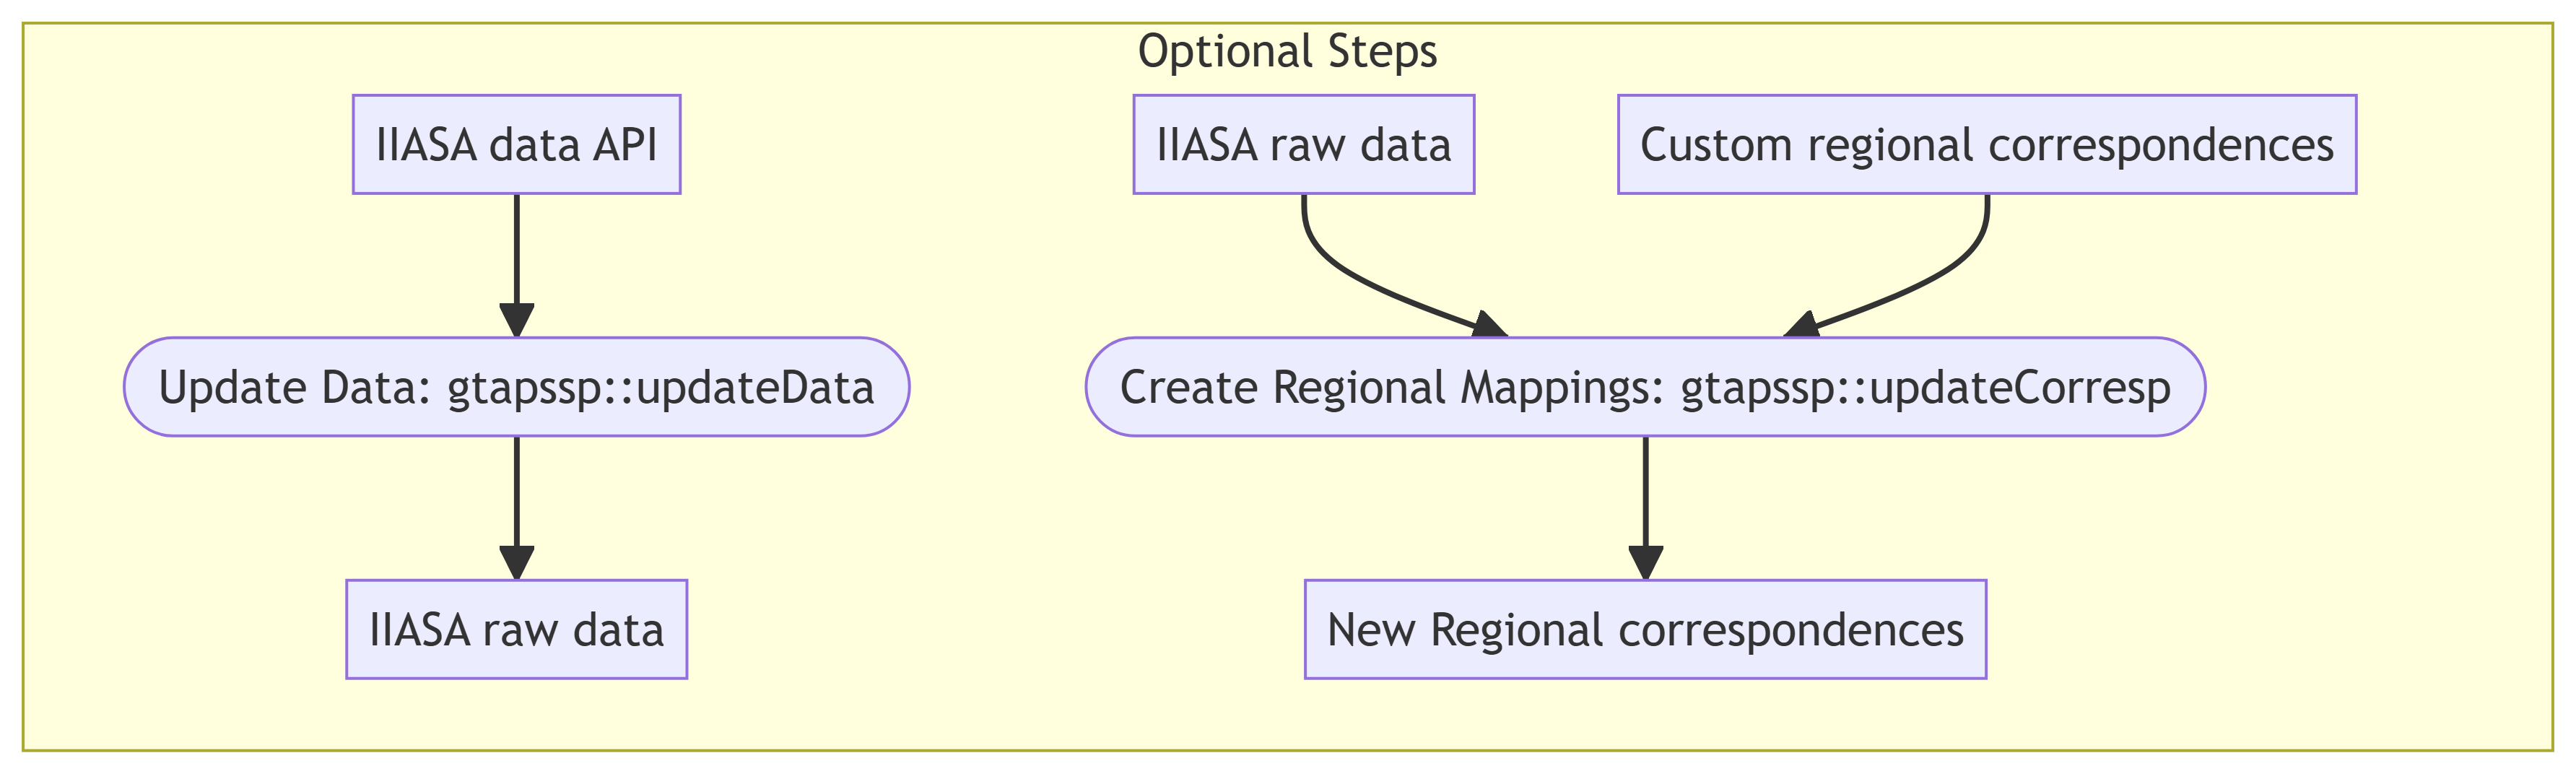
\includegraphics[width=9.29in,height=2.79in]{index_files/figure-latex/mermaid-figure-2.png}

To execute the functionality of updating data through the IIASA API, the
\href{https://rstudio.github.io/reticulate/}{reticulate} R package is
used as a bridge between the IIASA API (developed in Python) and the R
interface. However, it is essential to have Python installed on the
machine where the code will run. Additionally, the full path to the
\texttt{python.exe} executable must be provided to the
\texttt{gtapssp::updateData()} function, so R can access the installed
Python interpreter.

\begin{Shaded}
\begin{Highlighting}[]
\CommentTok{\# Ensure Python is installed on your machine}
\CommentTok{\# Configure the path to the python.exe executable}
\NormalTok{pythonExePath }\OtherTok{\textless{}{-}} \StringTok{"C:}\SpecialCharTok{\textbackslash{}\textbackslash{}}\StringTok{Users}\SpecialCharTok{\textbackslash{}\textbackslash{}}\StringTok{\textless{}username\textgreater{}}\SpecialCharTok{\textbackslash{}\textbackslash{}}\StringTok{AppData}\SpecialCharTok{\textbackslash{}\textbackslash{}}\StringTok{Local}\SpecialCharTok{\textbackslash{}\textbackslash{}}\StringTok{Programs}\SpecialCharTok{\textbackslash{}\textbackslash{}}\StringTok{Python}\SpecialCharTok{\textbackslash{}\textbackslash{}}\StringTok{Python312}\SpecialCharTok{\textbackslash{}\textbackslash{}}\StringTok{python.exe"}

\CommentTok{\# Use the gtapssp::updateData function to download and process updated data from IIASA}
\NormalTok{iiasa\_raw }\OtherTok{\textless{}{-}}\NormalTok{ gtapssp}\SpecialCharTok{::}\FunctionTok{updateData}\NormalTok{(}
  \AttributeTok{pythonExePath =}\NormalTok{ pythonExePath,}
  \AttributeTok{outputFile =} \StringTok{"data/iiasa\_raw.rda"} \CommentTok{\# Location to save the processed file}
\NormalTok{)}

\CommentTok{\# Funcion documentation:}
\NormalTok{?gtapssp}\SpecialCharTok{::}\NormalTok{updateData}
\end{Highlighting}
\end{Shaded}

You can also use the \texttt{gtapssp::updateCorresp()} function to apply
custom regional mappings, allowing flexibility to aggregate the dataset
according to your specific requirements.

\begin{Shaded}
\begin{Highlighting}[]
\CommentTok{\# Update regional correspondences}
\NormalTok{gtapssp}\SpecialCharTok{::}\FunctionTok{updateCorresp}\NormalTok{(}
  \AttributeTok{iiasa\_raw =}\NormalTok{ iiasa\_raw, }\CommentTok{\# or gtapssp::iiasa\_raw for use default input data}
  \AttributeTok{corresp\_reg =}\NormalTok{ gtapssp}\SpecialCharTok{::}\NormalTok{corresp\_reg }\CommentTok{\# or a custom vector of regional correspondences}
\NormalTok{)}

\CommentTok{\# Funcion documentation:}
\NormalTok{?gtapssp}\SpecialCharTok{::}\NormalTok{updateCorresp}
\end{Highlighting}
\end{Shaded}

The default regional mapping included in the package is displayed below.
This mapping aggregates the data to 251 regions using \texttt{reg\_iso3}
as the reference. However, it could be aggregated to the 160 GTAP
regions by using the \texttt{reg\_gtap\_code} column to agreggate
instead of \texttt{reg\_iso3.}

\begin{Shaded}
\begin{Highlighting}[]
\NormalTok{gtapssp}\SpecialCharTok{::}\NormalTok{corresp\_reg[, }\FunctionTok{c}\NormalTok{(}\StringTok{"reg\_iso3"}\NormalTok{, }\StringTok{"cty\_names"}\NormalTok{, }\StringTok{"reg\_gtap\_code"}\NormalTok{)]}
\end{Highlighting}
\end{Shaded}

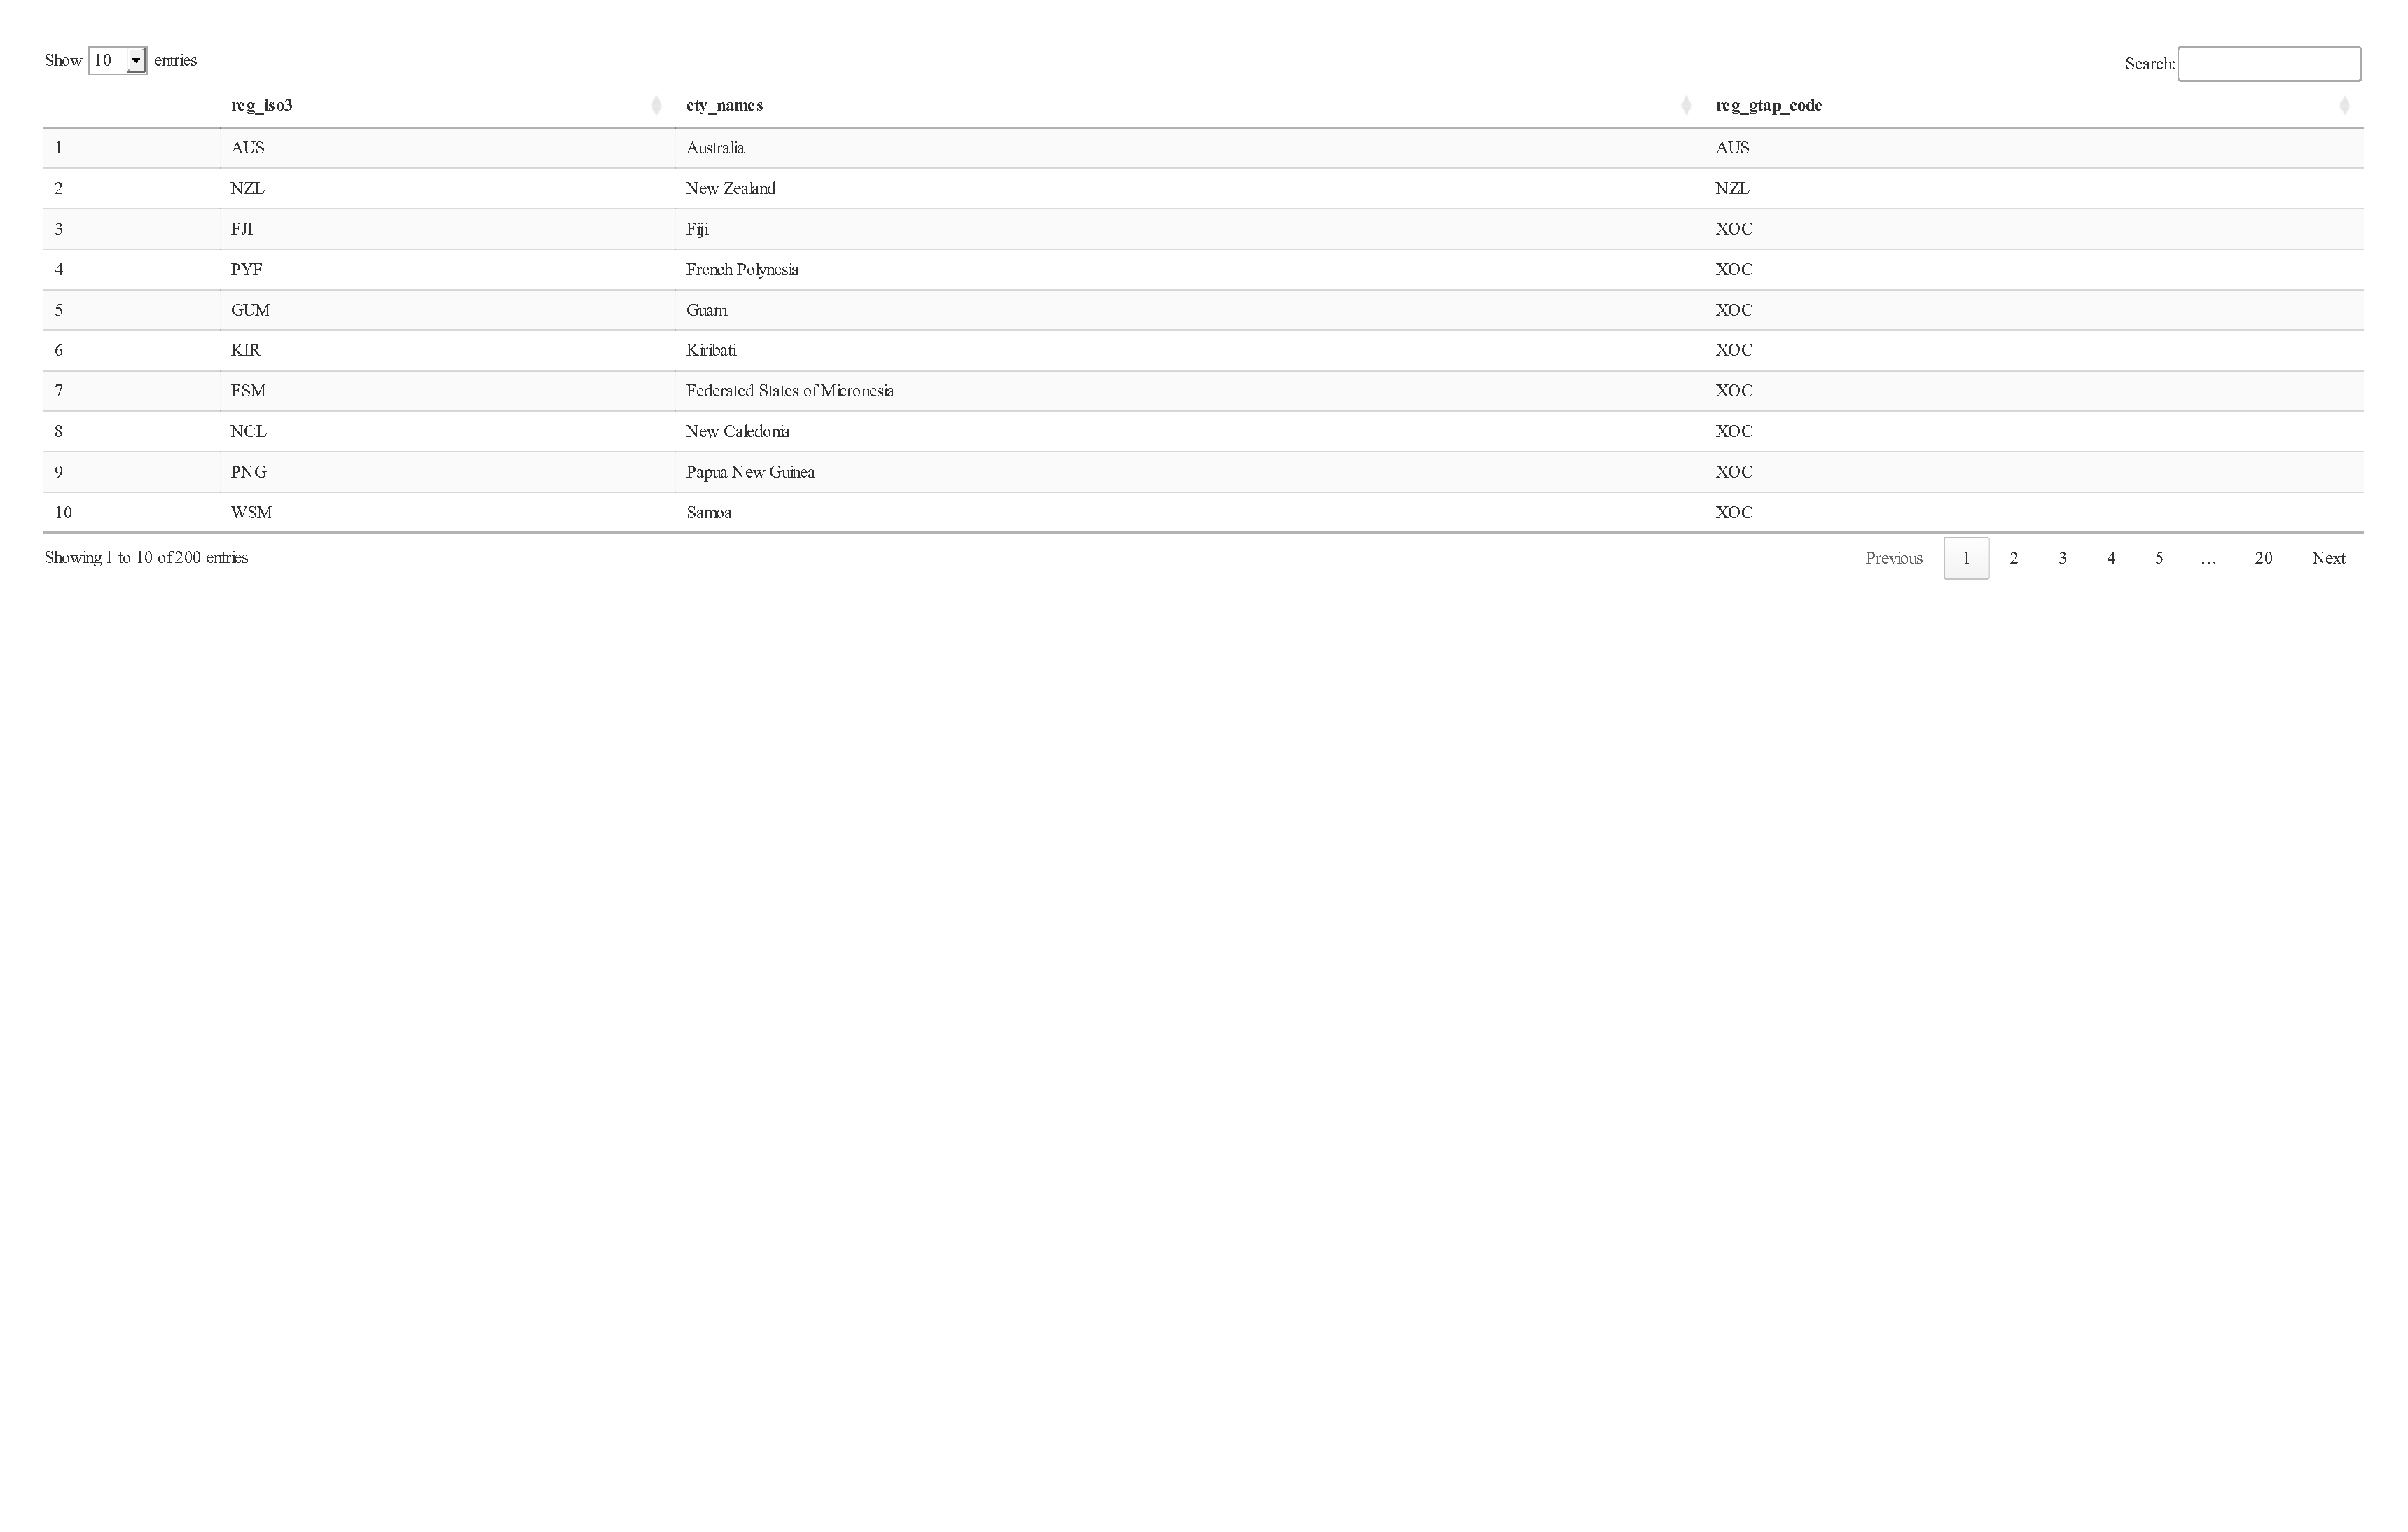
\includegraphics{index_files/figure-pdf/unnamed-chunk-32-1.pdf}

\section{Acknowledgments}\label{acknowledgments}

This tutorial and the development of the \texttt{gtapssp} package were
supported by the
\textbf{\href{https://www.gtap.agecon.purdue.edu/default.asp}{GTAP
Team}}, with special thanks to
\href{https://www.gtap.agecon.purdue.edu/network/member_display.asp?UserID=415}{\textbf{Dr.~Dominique
van der Mensbrugghe}},
\href{https://www.gtap.agecon.purdue.edu/network/member_display.asp?UserID=6446}{\textbf{Dr.~Angel
Aguiar}}, and
\href{https://www.gtap.agecon.purdue.edu/network/member_display.asp?UserID=2958}{\textbf{Dr.~Erwin
Corong}} for their guidance and expertise.




\end{document}
